\documentclass[11pt]{article}
\usepackage[a4paper,margin=1in]{geometry}
\usepackage{fancyhdr}
\usepackage{graphicx}
\usepackage{titlesec}
\usepackage{titling}
\usepackage{tocloft}
\usepackage{hyperref}
\usepackage{parskip}
\usepackage{xcolor}
\usepackage[rightcaption]{sidecap}
\usepackage{subcaption}
\usepackage{verbatim}
\usepackage{caption}
\usepackage{tabularx} 
\usepackage{amsmath}


% Setup header and footer
\pagestyle{fancy}
\fancyhf{}
\fancyhead[L]{Chiara Rizzi}
\fancyhead[R]{Natural Cycles Data Scientist Challenge}
\fancyfoot[C]{June 2025 \quad | \quad Page \thepage}

% Title formatting
\titleformat{\section}{\large\bfseries}{\thesection.}{0.5em}{}
\titleformat{\subsection}{\normalsize\bfseries}{\thesubsection.}{0.5em}{}

% Custom command for highlighting questions
\newcommand{\questiontext}[1]{\vspace{0.5em}\textbf{\textit{\textcolor{gray}{#1}}}}

% Document title
\title{
  \textbf{Natural Cycles Data Scientist Challenge} \\
  \large Chiara Rizzi \\
  \vspace{0.3cm}
  \normalsize\textit{Code available at \url{https://github.com/chiara-rizzi/natural-cycles-assignment}}
}\date{June 2025}

\begin{document}

\maketitle
\thispagestyle{fancy}

\tableofcontents
\newpage

\paragraph{Disclaimer.} This work was informed by the paper \textit{Time to Pregnancy for Women Using a Fertility Awareness Based Mobile Application to Plan a Pregnancy} by Favaro et al.\ (Journal of Women's Health, 2021), which I had read prior to the HR interview. 
All analytical work, as well as the structure and content of this report, are entirely my own. ChatGPT was used to refine the final language and to clean up the codebase prior to submission.


\vspace{1em}

\section{Summary of Results}

\questiontext{What is the chance of getting pregnant within 13 cycles?}

Using \textbf{Kaplan–Meier survival analysis}, which accounts for censored observations, I estimated that the probability of getting pregnant within 13 cycles is \textbf{75\%}. The 95\% confidence interval for this estimate is \textbf{[72\%, 77\%]}. More details in Section \ref{sec:time-to-event}.


\questiontext{How long does it usually take to get pregnant?}

The Kaplan–Meier survival analysis estimated a median time to pregnancy of \textbf{5 cycles}. More details in Section \ref{sec:time-to-event}.


\questiontext{What factors impact the time it takes to get pregnant?}

I estimated the factors that have a statistically significant impact on the time to pregnancy using a \textbf{discrete-time proportional odds regression model}. Missing values were imputed using MICE with LightGBM. Higher \textbf{age} and \textbf{being underweight} were associated with lower odds of conception (OR~$<$~1), while \textbf{previous pregnancies}, more \textbf{dedicated use of the NC app}, and higher \textbf{frequency of logged intercourse} were associated with higher odds (OR~$>$~1). These findings were confirmed using a Cox proportional hazards model. More details in Section \ref{sec:other_factors}.

\questiontext{How would your approach change if you were to use different techniques (e.g., ML or non-ML methods)? What trade-offs would you consider?}

Except for the imputation of missing data, I did not use machine learning (ML) in this assignment, as traditional survival analysis methods were more appropriate for inference and uncertainty estimation in Questions 1 and 2. ML is more suitable for individual-level prediction and requires models that handle censored data. For Question 3, techniques like Random Survival Forests or \texttt{DeepSurv} could be valid when assumptions of traditional models are violated. I chose classical methods for their interpretability and ability to estimate confidence intervals. More details in Section \ref{sec:thoughts}

\vspace{1em}


\section{Exploratory Data Analysis}
\label{sec:eda}

I started with an exploratory data analysis (EDA) to understand the main characteristics of the dataset. The EDA was guided by the questions of the assignment, and includes some early qualitative observations related to them. A more rigorous statistical treatment is presented in the following sections.

Two key variables in the dataset are the number of cycles in the attempt to conceive (\texttt{n\_cycles\_trying}) and the final outcome (\texttt{outcome}).

\begin{itemize}
    \item The dataset contains observations for 1995 women.
    \item 1148 of them achieved pregnancy during the observed period.
    \item All pregnancies occurred within 13 cycles.
    \item 847 did not achieve pregnancy during the observed period.
    \item For 683 of these 847 women, the observed period was shorter than 13 cycles (e.g., due to discontinuing use of the NC app), meaning they might still have conceived within 13 cycles.
\end{itemize}

From these numbers, I derived simple bounds for the probability of getting pregnant within 13 cycles: the value lies between \textbf{58\% and 92\%}, depending on whether we assume none or all of the 683 shorter-observed users would have eventually conceived.

Figure~\ref{fig:n_cycles_trying__outcome_pregnant_1} shows the distribution of \texttt{n\_cycles\_trying} for the 1148 women who became pregnant. The median is 2 cycles and the mean is 3.38. However, these statistics are not reliable estimates of typical time to pregnancy, as they exclude censored data (women for whom the outcome of the attempt is not fully observed, e.g. because they discontinued the usage of the app), a key limitation that will be addressed later.

\begin{SCfigure}[1.0][h]
  \centering
  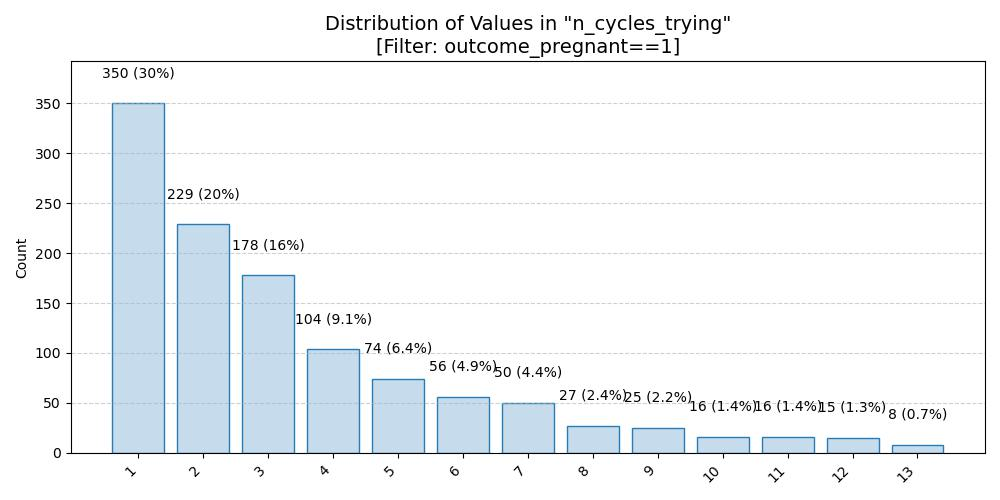
\includegraphics[width=0.65\linewidth]{plots/n_cycles_trying__outcome_pregnant_1.jpg}
  \caption{
    Distribution of the number of cycles in the attempt to conceive (\texttt{n\_cycles\_trying}) for women who achieved pregnancy within the observed time.\\} 
    \label{fig:n_cycles_trying__outcome_pregnant_1}
\end{SCfigure}

To better understand the data structure, I looked at missing values across all variables. Figure~\ref{fig:missing_values} shows the number of missing values for each. Overall, the dataset is well populated: the variable with the most missing values is \texttt{sleeping\_pattern}, with around 25\% missing. It’s also worth noting that, while not technically missing, \texttt{dedication} and \texttt{intercourse\_frequency} often have a value zero, which corresponds to no activity logged by the user. This occurs in 13\% and 19\% of the entries, respectively.

\begin{SCfigure}[1.0][h]
  \centering
  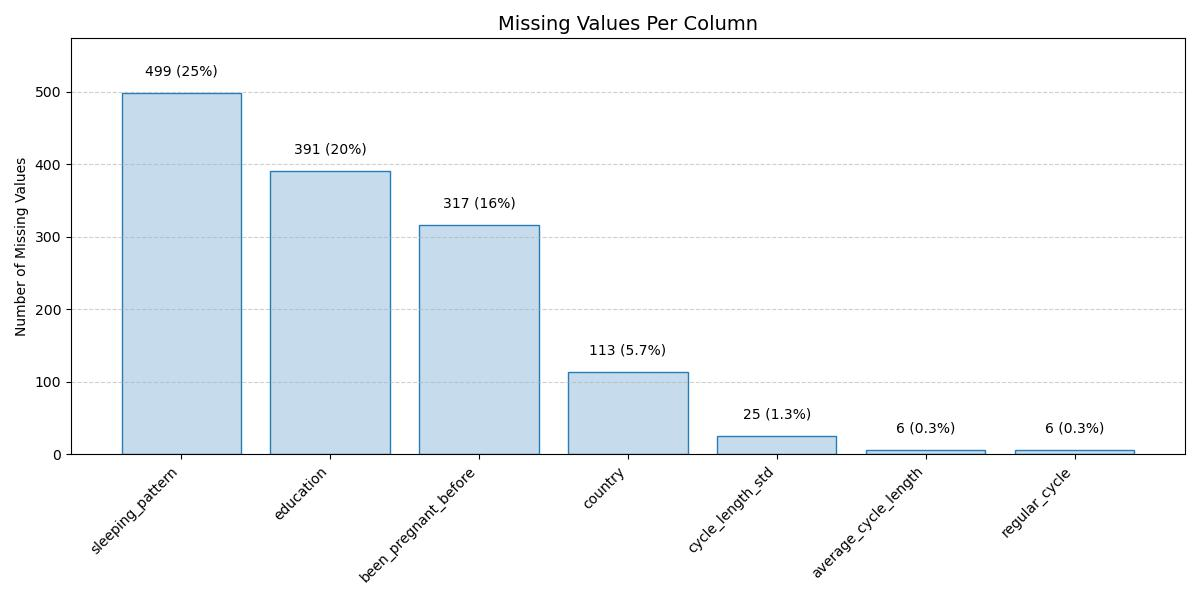
\includegraphics[width=0.65\linewidth]{plots/missing_values.jpg}
  \caption{
  Number of missing values for the variables in the dataset.\\
  } 
    \label{fig:missing_values}
\end{SCfigure}

I explored the distributions of all categorical and numerical variables; these are available in Appendix~\ref{app:variables} for reference.

To examine relationships between variables, I computed a Pearson correlation matrix. Since many variables are categorical, I encoded them numerically where it made conceptual sense, in order to calculate correlations. While dedicated methods exist for assessing associations between categorical variables, for this exploratory phase I prioritized simplicity. The encoding used is reported in Table~\ref{tab:ordered_encodings}.

\begin{table}[h]
\centering
\caption{Encoding of ordered categorical variables used to study correlations.}
\label{tab:ordered_encodings}
\begin{tabularx}{\textwidth}{X X X}
\textbf{Education Level} & \textbf{Sleeping Pattern} & \textbf{Pregnancy History} \\
\hline
0 – Elementary school & 0 – Several times during the night & 0 – No, never \\
1 – High school & 1 – Shift worker & 1 – Yes, once \\
2 – Trade / technical / vocational training & 2 – Late and snoozer & 2 – Yes, twice \\
3 – University & 3 – Wake same every workday & 3 – Yes 3 times or more \\
4 – PhD & 4 – Wake same every day & \\
\end{tabularx}
\end{table}

The resulting correlation matrix is shown in Figure~\ref{fig:correlation_matrix}. Because censored data are not accounted for here, correlations involving \texttt{n\_cycles\_trying} and \texttt{outcome} should be interpreted cautiously. Nonetheless, the matrix reveals useful patterns. Focusing on correlations above 20\%, we see a positive association between \texttt{age} and both \texttt{education} level (29\%) and \texttt{been\_pregnant\_before} (27\%). As expected, longer \texttt{average\_cycle\_length} is associated with less regular \texttt{regular\_cycle}, and higher \texttt{dedication} is positively correlated with \texttt{intercourse\_frequency} (47\%).

\begin{SCfigure}[1.0][h]
  \centering
  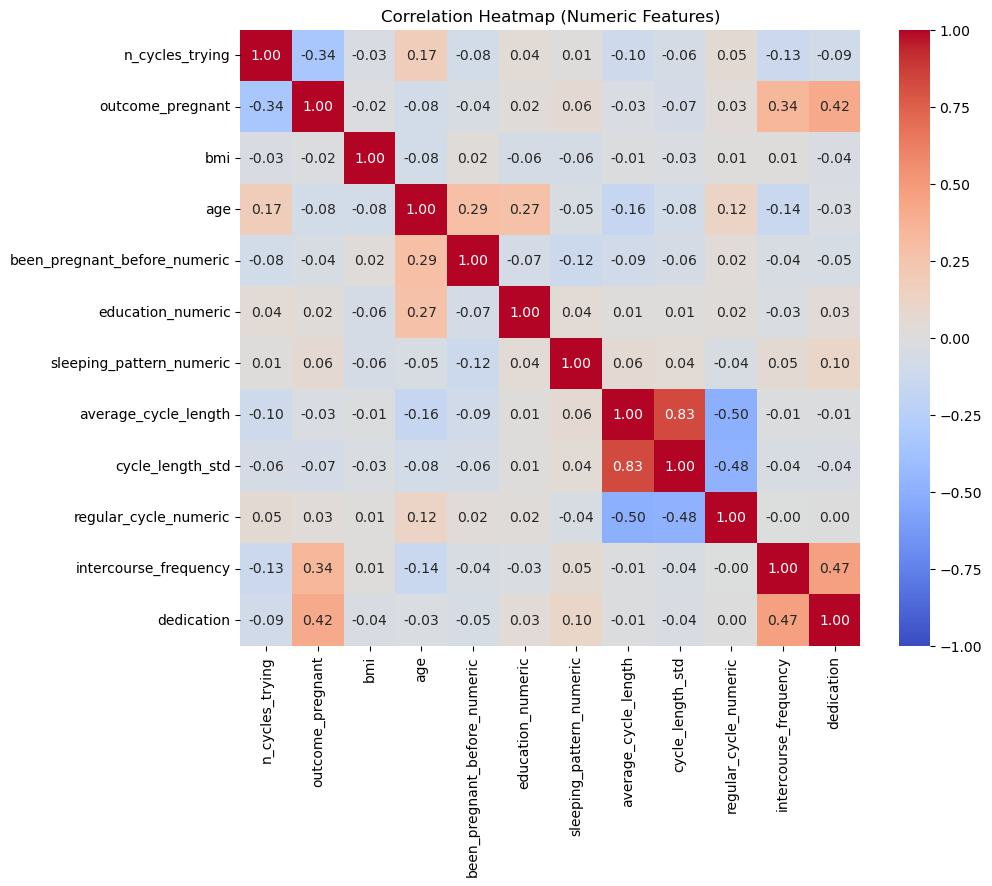
\includegraphics[width=0.65\linewidth]{plots/correlation_matrix_new_variables.jpg}
  \caption{
  Correlation matrix for the numerical variables and the encoded categorical ones.\\
  } 
    \label{fig:correlation_matrix}
\end{SCfigure}

Finally, I examined correlations restricted to users who became pregnant (Figure~\ref{fig:correlation_matrix_new_variables_outcome_pregnant}). This gives a qualitative sense of which variables may affect time to pregnancy, by observing correlations with \texttt{n\_cycles\_trying}. While again this ignores censored data, a few patterns emerge: time to pregnancy increases with \texttt{age}, and decreases with \texttt{been\_pregnant\_before}, \texttt{dedication}, and \texttt{intercourse\_frequency}. These findings provide useful intuition, and will be explored more rigorously in Section~\ref{sec:other_factors}.

\begin{SCfigure}[1.0][h]
  \centering
  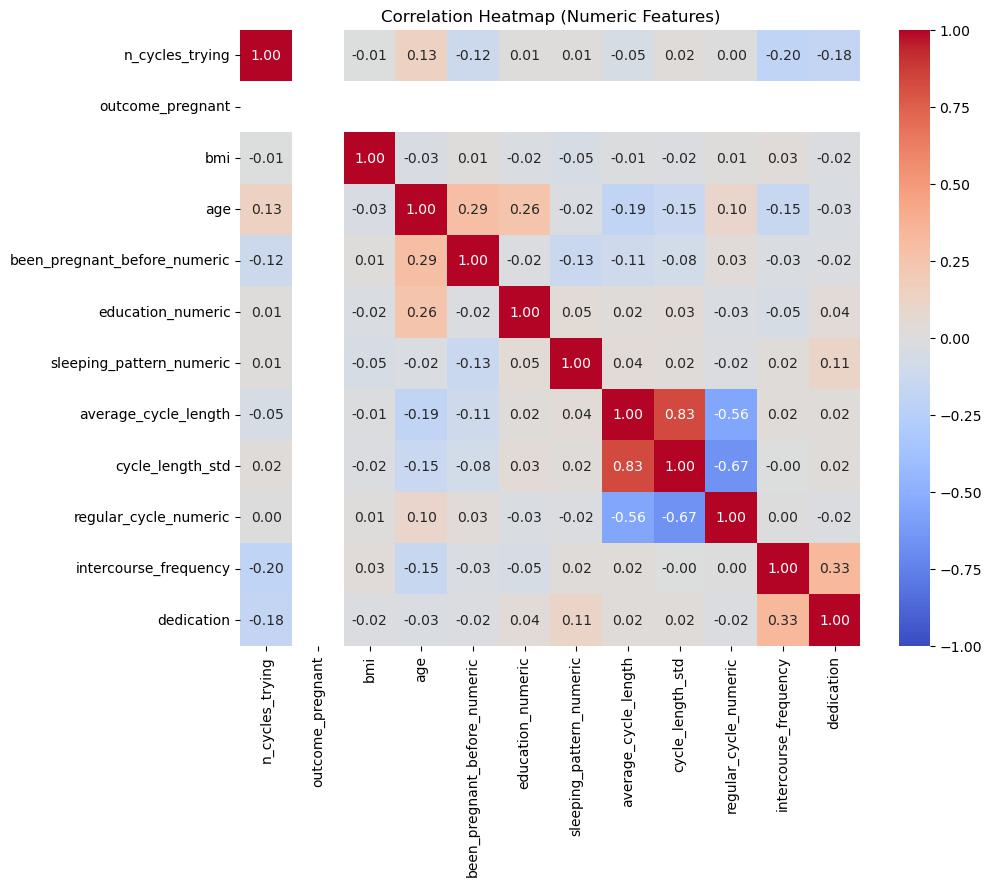
\includegraphics[width=0.65\linewidth]{plots/correlation_matrix_new_variables_outcome_pregnant.jpg}
  \caption{
  Correlation matrix restricted to users who reported a pregnancy.\\
  } 
    \label{fig:correlation_matrix_new_variables_outcome_pregnant}
\end{SCfigure}

I chose to exclude the variable \textit{country} from the analysis because I do not expect it to have a strong impact on time to pregnancy and believe it mostly reflects patterns of adoption of the NC app. Including it could also add unnecessary noise to the analysis.






\section{Questions 1 and 2: Time-to-Event Analysis}
\label{sec:time-to-event}
\questiontext{What is the chance of getting pregnant within 13 cycles?}

To answer this question, I used survival analysis, specifically the Kaplan–Meier estimator, a standard approach for time-to-event data. In this context, the duration is the discrete number of cycles, and the event is pregnancy. This method accounts for censored observations by incorporating each woman's data for the full duration she was observed, regardless of whether she conceived.

The analysis was implemented in \textit{Python}, using the \texttt{KaplanMeierFitter} class from the \texttt{lifelines} library.

I found that the estimated probability of getting pregnant within 13 cycles is \textbf{75\%}. The corresponding 95\% confidence interval, calculated using Greenwood's formula and a log-minus-log transformation, is \textbf{[72\%, 77\%]}. This value was computed as one minus the estimated survival probability at cycle 13 — that is, the probability of not yet being pregnant by that point.

The survival function is shown in Figure~\ref{fig:km_survival}.

\begin{SCfigure}[1.0][h]
  \centering
  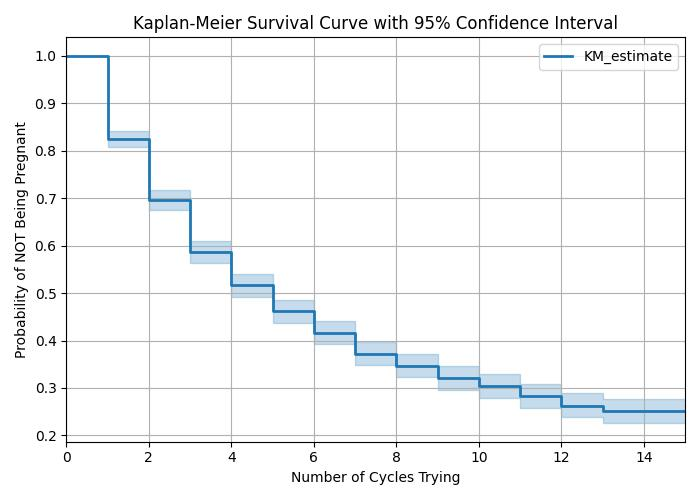
\includegraphics[width=0.65\linewidth]{plots/Q1_survival_curve.jpg}
  \caption{
    Survival function of time to pregnancy, estimated using the Kaplan–Meier estimator. The shaded area represents the 95\% confidence interval.\\} 
    \label{fig:km_survival}
\end{SCfigure}

The survival curve shows that the likelihood of pregnancy is highest during the first few cycles and gradually decreases over time. The confidence bands are narrow in the early cycles and widen in later cycles, reflecting greater uncertainty due to censoring and the decreasing number of women remaining under observation at each cycle.

\questiontext{How long does it usually take to get pregnant?}

A natural estimate for how long it typically takes to get pregnant is the median survival time. In this case, the estimated \textbf{median number of cycles to pregnancy is 5}. 


\section{Question 3: Factors That Impact the Time It Takes to Get Pregnant}
\label{sec:other_factors}

\questiontext{What factors impact the time it takes to get pregnant?}

This question was the most interesting to explore, as unlike the previous ones, there isn’t a single natural modeling choice — multiple valid approaches are possible depending on how time and interpretation are treated.

My main method was a \textbf{discrete-time proportional odds logistic regression model}, and I verified the results using a \textbf{Cox proportional hazards model}. Both are commonly used in survival analysis. The main difference lies in how they handle time — one works in discrete steps (cycles), the other assumes continuous time — and how the results are interpreted: in terms of odds ratios for the former, and hazard ratios for the latter.

I chose the discrete-time model as the primary approach because it naturally fits this problem, where time is measured in cycles. The Cox model, widely used in medical research, complements it well and provides a useful comparison.


\subsection{Treatment of Missing Values}

As discussed in Section~\ref{sec:eda}, the variables related to additional factors that may influence the time to pregnancy (TTP) exhibit varying levels of missing data, ranging from 0\% to 25\%. The three variables with the highest percentages of missing values are:

\begin{itemize}
    \item \texttt{sleeping\_pattern}: 25\%
    \item \texttt{education}: 20\%
    \item \texttt{been\_pregnant\_before}: 16\%
\end{itemize}

As a first step, I ran the analysis described in the following subsections using only complete cases — i.e., retaining only those entries with no missing values in the variables of interest. This resulted in the removal of 751 entries, leaving 1244 complete cases in the observed dataset.

The outcome of this initial analysis, shown in Appendix~\ref{app:missing_variables}, indicated that among the three variables with higher levels of missingness, only \texttt{been\_pregnant\_before} had a notable impact on TTP. This highlighted the need to handle this variable with particular care during imputation.

To address missing values, I used multivariate imputation via the \texttt{miceforest} Python library, which implements the Multiple Imputation by Chained Equations (MICE) algorithm using LightGBM (gradient-boosted decision trees). Categorical variables were encoded numerically following the scheme shown in Table~\ref{tab:ordered_encodings}.

I opted for this approach over simpler methods (e.g., random or mode imputation) to preserve the correlation structure present in the data. In particular, as shown in the correlation matrix in Section~\ref{sec:eda} (Figure~\ref{fig:correlation_matrix}), \texttt{been\_pregnant\_before} is correlated with \texttt{age}. Preserving this relationship was important to avoid biasing the results.

I ran \texttt{miceforest} for 50 iterations, starting from the numerically encoded variables, and verified that the distributions of imputed values were statistically consistent with the original ones. Distribution comparisons are shown in Appendix~\ref{app:missing_variables}.

This imputation approach allowed me to retain the full dataset, reducing statistical uncertainty in the final results.

It is worth noting that the benefits of this approach could be extended further by performing the analysis across multiple imputed datasets and pooling the results to account for imputation variability. This was not done here due to time constraints.




\subsection{Categories and Baseline Group}

Both discrete-time proportional odds logistic regression and Cox models can accept continuous or categorical variables. To simplify interpretation, I encoded all variables as categorical by grouping continuous ones based on their values. This made it easier to define a baseline group, and to interpret model outputs as odds ratios (or hazard ratios) relative to that group.

For binary variables like \texttt{regular\_cycle}, the dataset already provided categorical values. For others:

\begin{itemize}
  \item \texttt{age}, \texttt{dedication}, and \texttt{intercourse\_frequency} were divided into three groups: a central group containing 50\% of entries, and two outer groups with 25\% each.
  \item \texttt{bmi} was categorized using WHO guidelines: underweight (BMI~$<$~18), normal (BMI 18--25), and overweight (BMI~$>$~25).
  \item \texttt{average\_cycle\_length} was labeled "normal" if between 21 and 35 days. Durations outside this range have been grouped together due to the low statistics.
  \item \texttt{regular\_cycle} was defined in the dataset based on a cycle length standard deviation below 5 days.
\end{itemize}

For \texttt{dedication} and \texttt{intercourse\_frequency}, I considered whether to treat the value zero (indicating no data logged) as a separate category. For simplicity, I included these cases in the "low" group.

The \textbf{baseline group} includes women aged 30--35, with normal BMI, regular cycles between 21 and 35 days, who have never been pregnant, do not have university-level education, report regular sleep patterns, and have medium levels of both BBT logging (\texttt{dedication}) and \texttt{intercourse\_frequency}. 

Table~\ref{tab:model_encodings} summarizes the grouping strategy and the baseline category for each variable.



\begin{table}[h]
\centering
\caption{Categorical encodings used for modeling. Baseline categories are shown in \textcolor{blue}{\textbf{bold blue}}.}
\label{tab:model_encodings}

% First row
\begin{tabularx}{\textwidth}{X X X}
\textbf{Age [years]} & \textbf{BMI} & \textbf{Pregnancy History} \\
\hline
19--29 & Underweight & True \\
\textcolor{blue}{\textbf{30--35}} & \textcolor{blue}{\textbf{Normal}} & \textcolor{blue}{\textbf{False}} \\
36--44 & Overweight & \\
\end{tabularx}
\vspace{1em}

% Second row
\begin{tabularx}{\textwidth}{X X X}
\textbf{Cycle Length [days]} & \textbf{Regular Cycle} & \textbf{University Education} \\
\hline
\textcolor{blue}{\textbf{21--35}} & \textcolor{blue}{\textbf{True}} & True \\
\(<21\) OR \(>35\) & False & \textcolor{blue}{\textbf{False}} \\
 & & \\
\end{tabularx}
\vspace{1em}

% Third row
\begin{tabularx}{\textwidth}{X X X}
\textbf{Regular Sleep} & \textbf{Intercourse Frequency} & \textbf{Dedication Level} \\
\hline
\textcolor{blue}{\textbf{True}} & Low & Low \\
False & \textcolor{blue}{\textbf{Medium}} & \textcolor{blue}{\textbf{Medium}} \\
& High & High \\
\end{tabularx}

\vspace{1em}

\captionsetup{justification=justified}
%\caption*{\textit{Note}: “Low” intercourse frequency = fewer than \textit{X} times/month; “Medium” = \textit{Y–Z}; “High” = more than \textit{Z}. Dedication levels are based on self-tracking frequency and consistency with lifestyle targets.}
\end{table}


\subsection{Discrete-Time Proportional Odds Logistic Regression Model}

For the discrete-time proportional odds regression model, the dataset must be transformed into a "long" format, with one row for each individual and each cycle they were observed. This structure requires an additional variable that tracks the specific cycle number (not just the total number of cycles observed). This is necessary to properly model the cycle-dependent nature of conception probability — as noted earlier, earlier cycles tend to have a higher per-cycle chance of pregnancy.

To stabilize model fitting while preserving this time dependence, I grouped the cycle variable into five bins: \texttt{1--3}, \texttt{4--6}, \texttt{7--9}, \texttt{10--12}, and \texttt{13+}.

The model was implemented using the \texttt{Logit} function from the \texttt{statsmodels} library in \textit{Python}. Odds ratios (ORs) and their 95\% confidence intervals (CIs) were computed by exponentiating the model coefficients and their standard errors:

\begin{equation*}
\begin{aligned}
\text{CI Lower} &= \exp\left(\text{Coef.} - 1.96 \times \text{Std.Err.}\right) \\
\text{CI Upper} &= \exp\left(\text{Coef.} + 1.96 \times \text{Std.Err.}\right)
\end{aligned}
\end{equation*}

Appendix~\ref{app:survival_subgroups} contains a visual assessment of whether the proportional odds assumption holds.

Figure~\ref{fig:or} shows the estimated odds ratios for each covariate, along with their confidence intervals. Variables with odds ratios significantly different from 1 are highlighted in red.

As anticipated qualitatively in Section~\ref{sec:eda}, the model indicates that \textbf{higher age is associated with reduced odds of pregnancy}, while \textbf{previous pregnancies}, \textbf{more dedicated app usage}, and \textbf{higher frequency of logged intercourse} are associated with increased odds. The analysis also highlights that \textbf{being underweight may negatively impact the per-cycle chances of conception}.


\begin{SCfigure}[1.0][h]
  \centering
  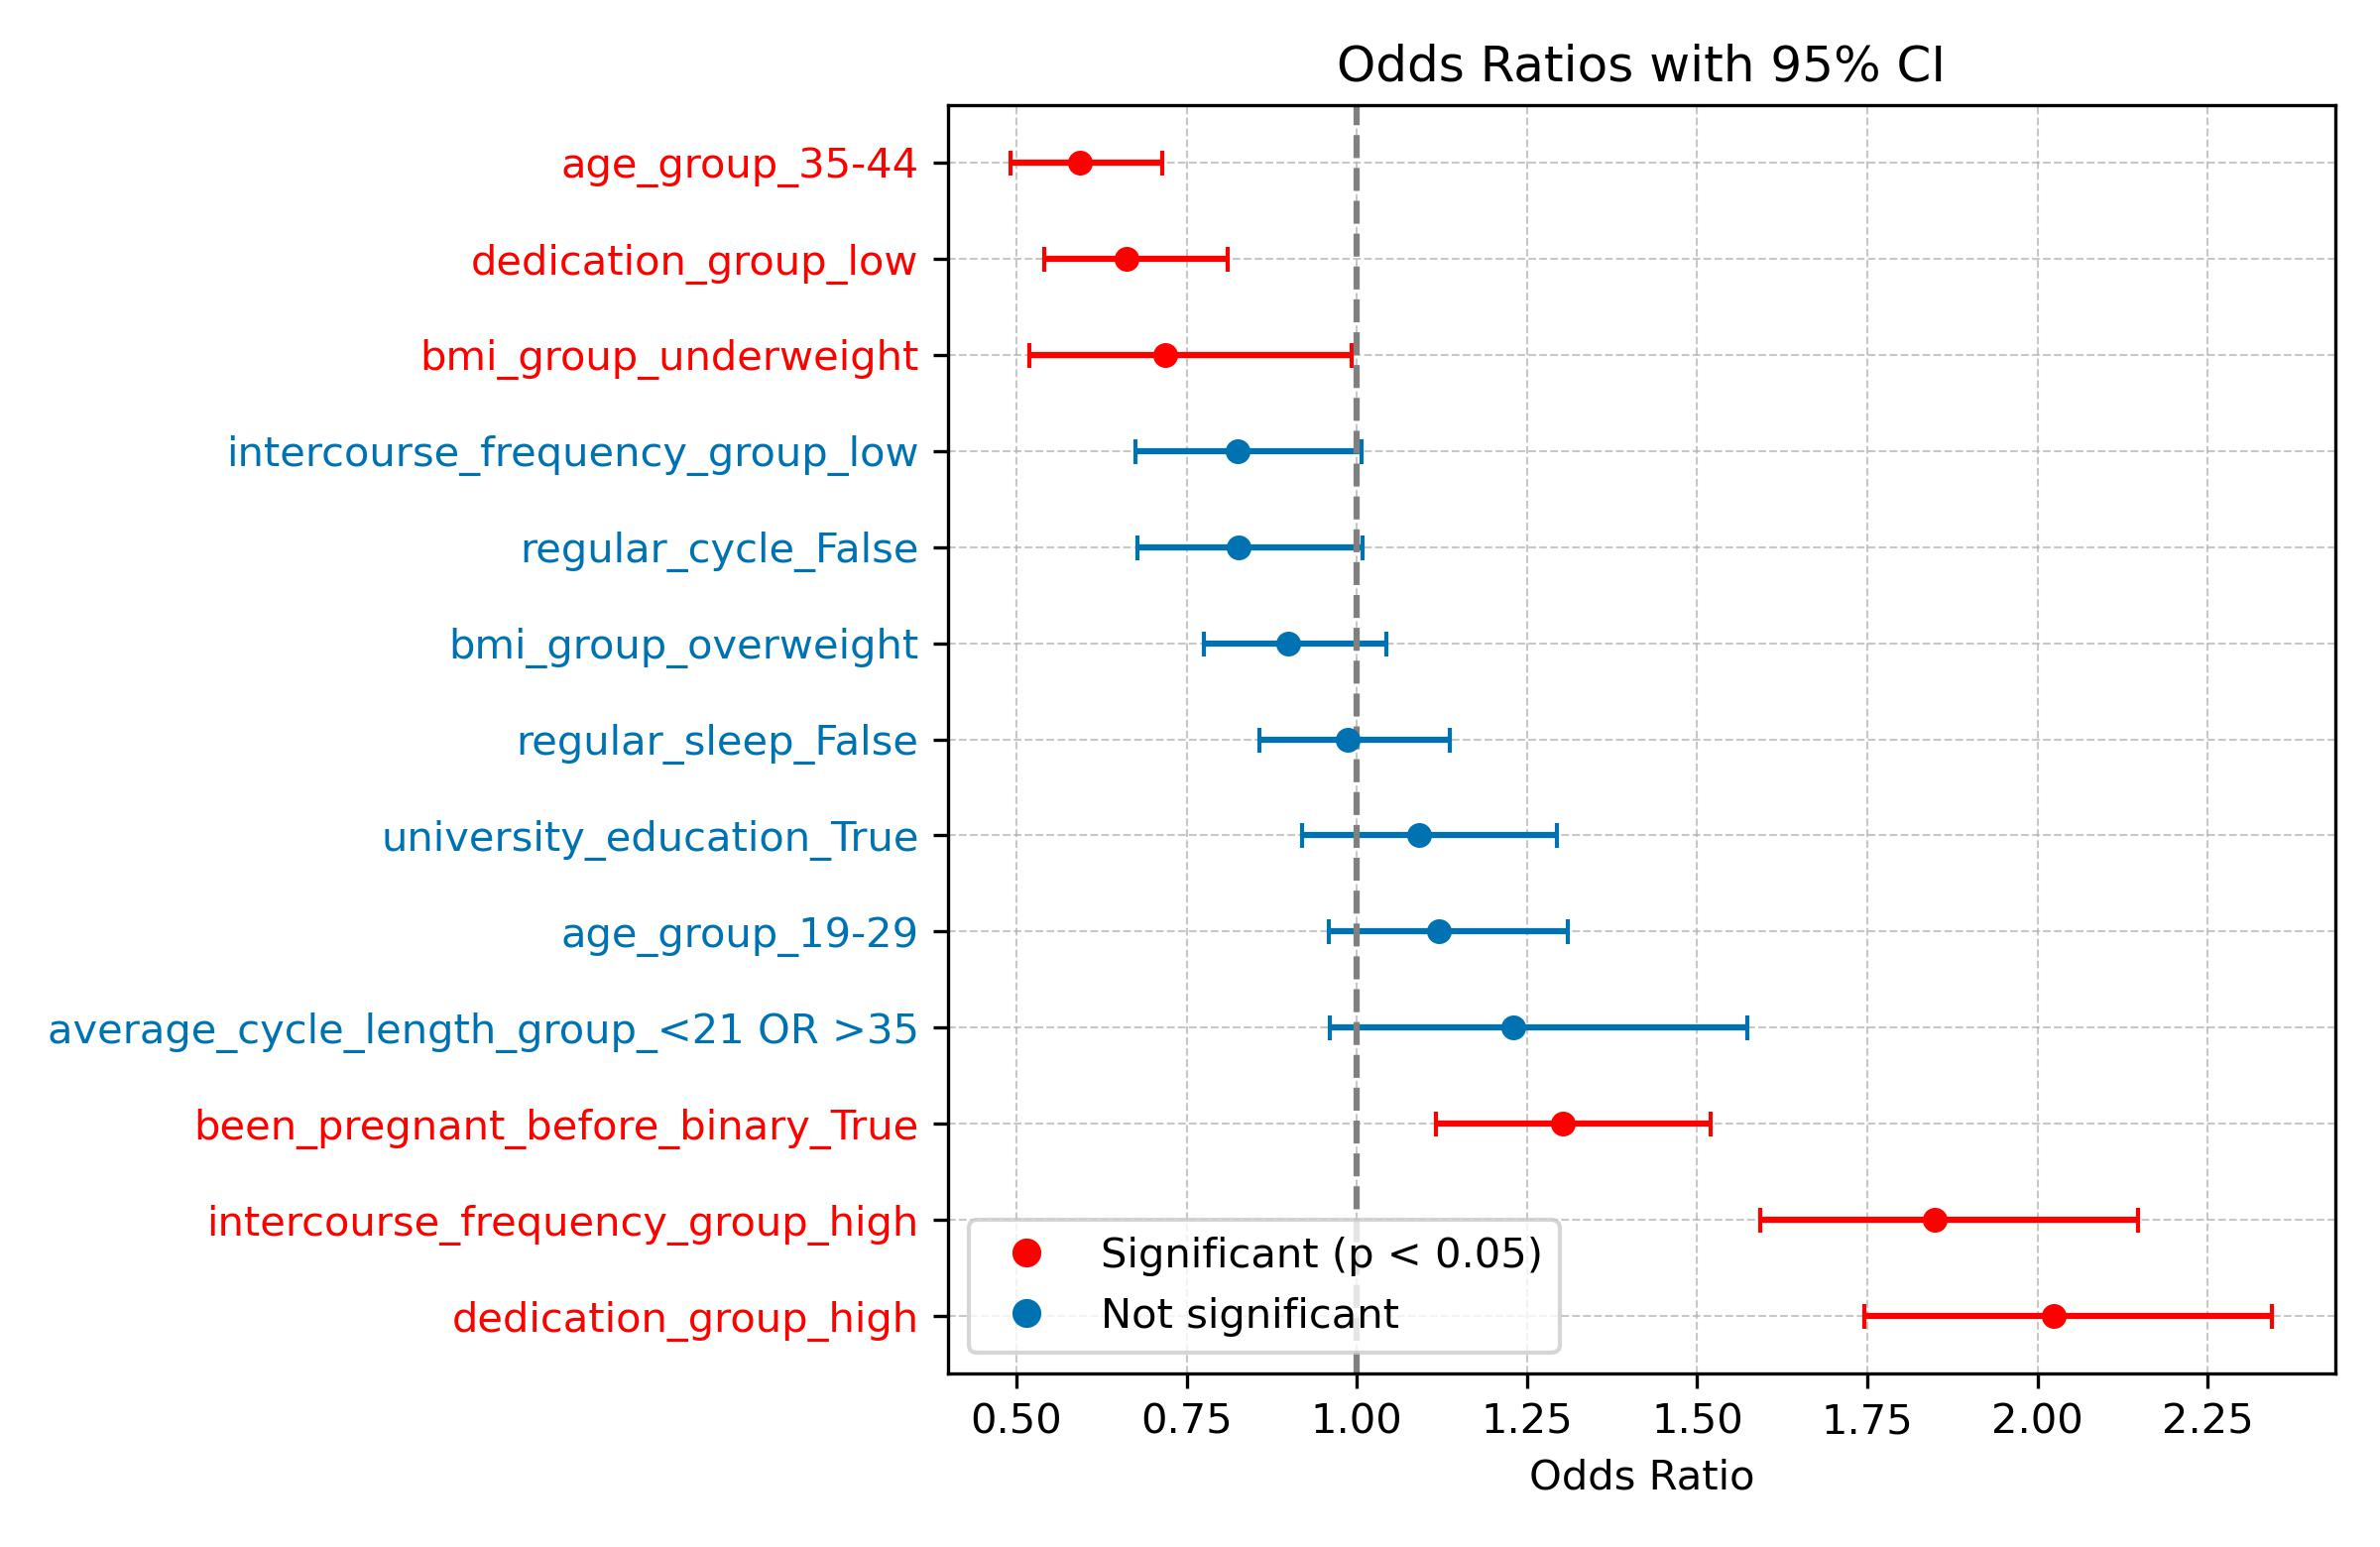
\includegraphics[width=0.65\linewidth]{plots/OR.jpg}
  \caption{
    Odds ratios for factors potentially affecting time to pregnancy, estimated using a discrete-time proportional odds regression model. Red bars indicate variables with statistically significant effects. \\
  } 
  \label{fig:or}
\end{SCfigure}


\subsection{Cox Proportional Hazards Model}

I carried out the Cox proportional hazards model analysis of the factors influencing time to pregnancy (TTP) using \textit{Python} and the \texttt{CoxPHFitter} class from the \texttt{lifelines} library. Hazard ratios (HRs) and their 95\% confidence intervals (CIs) were computed by exponentiating the model coefficients and their respective CIs.

The estimated HRs are shown in Figure~\ref{fig:cox_hr}, with values significantly different from 1 highlighted in red.

\begin{SCfigure}[1.0][h]
  \centering
  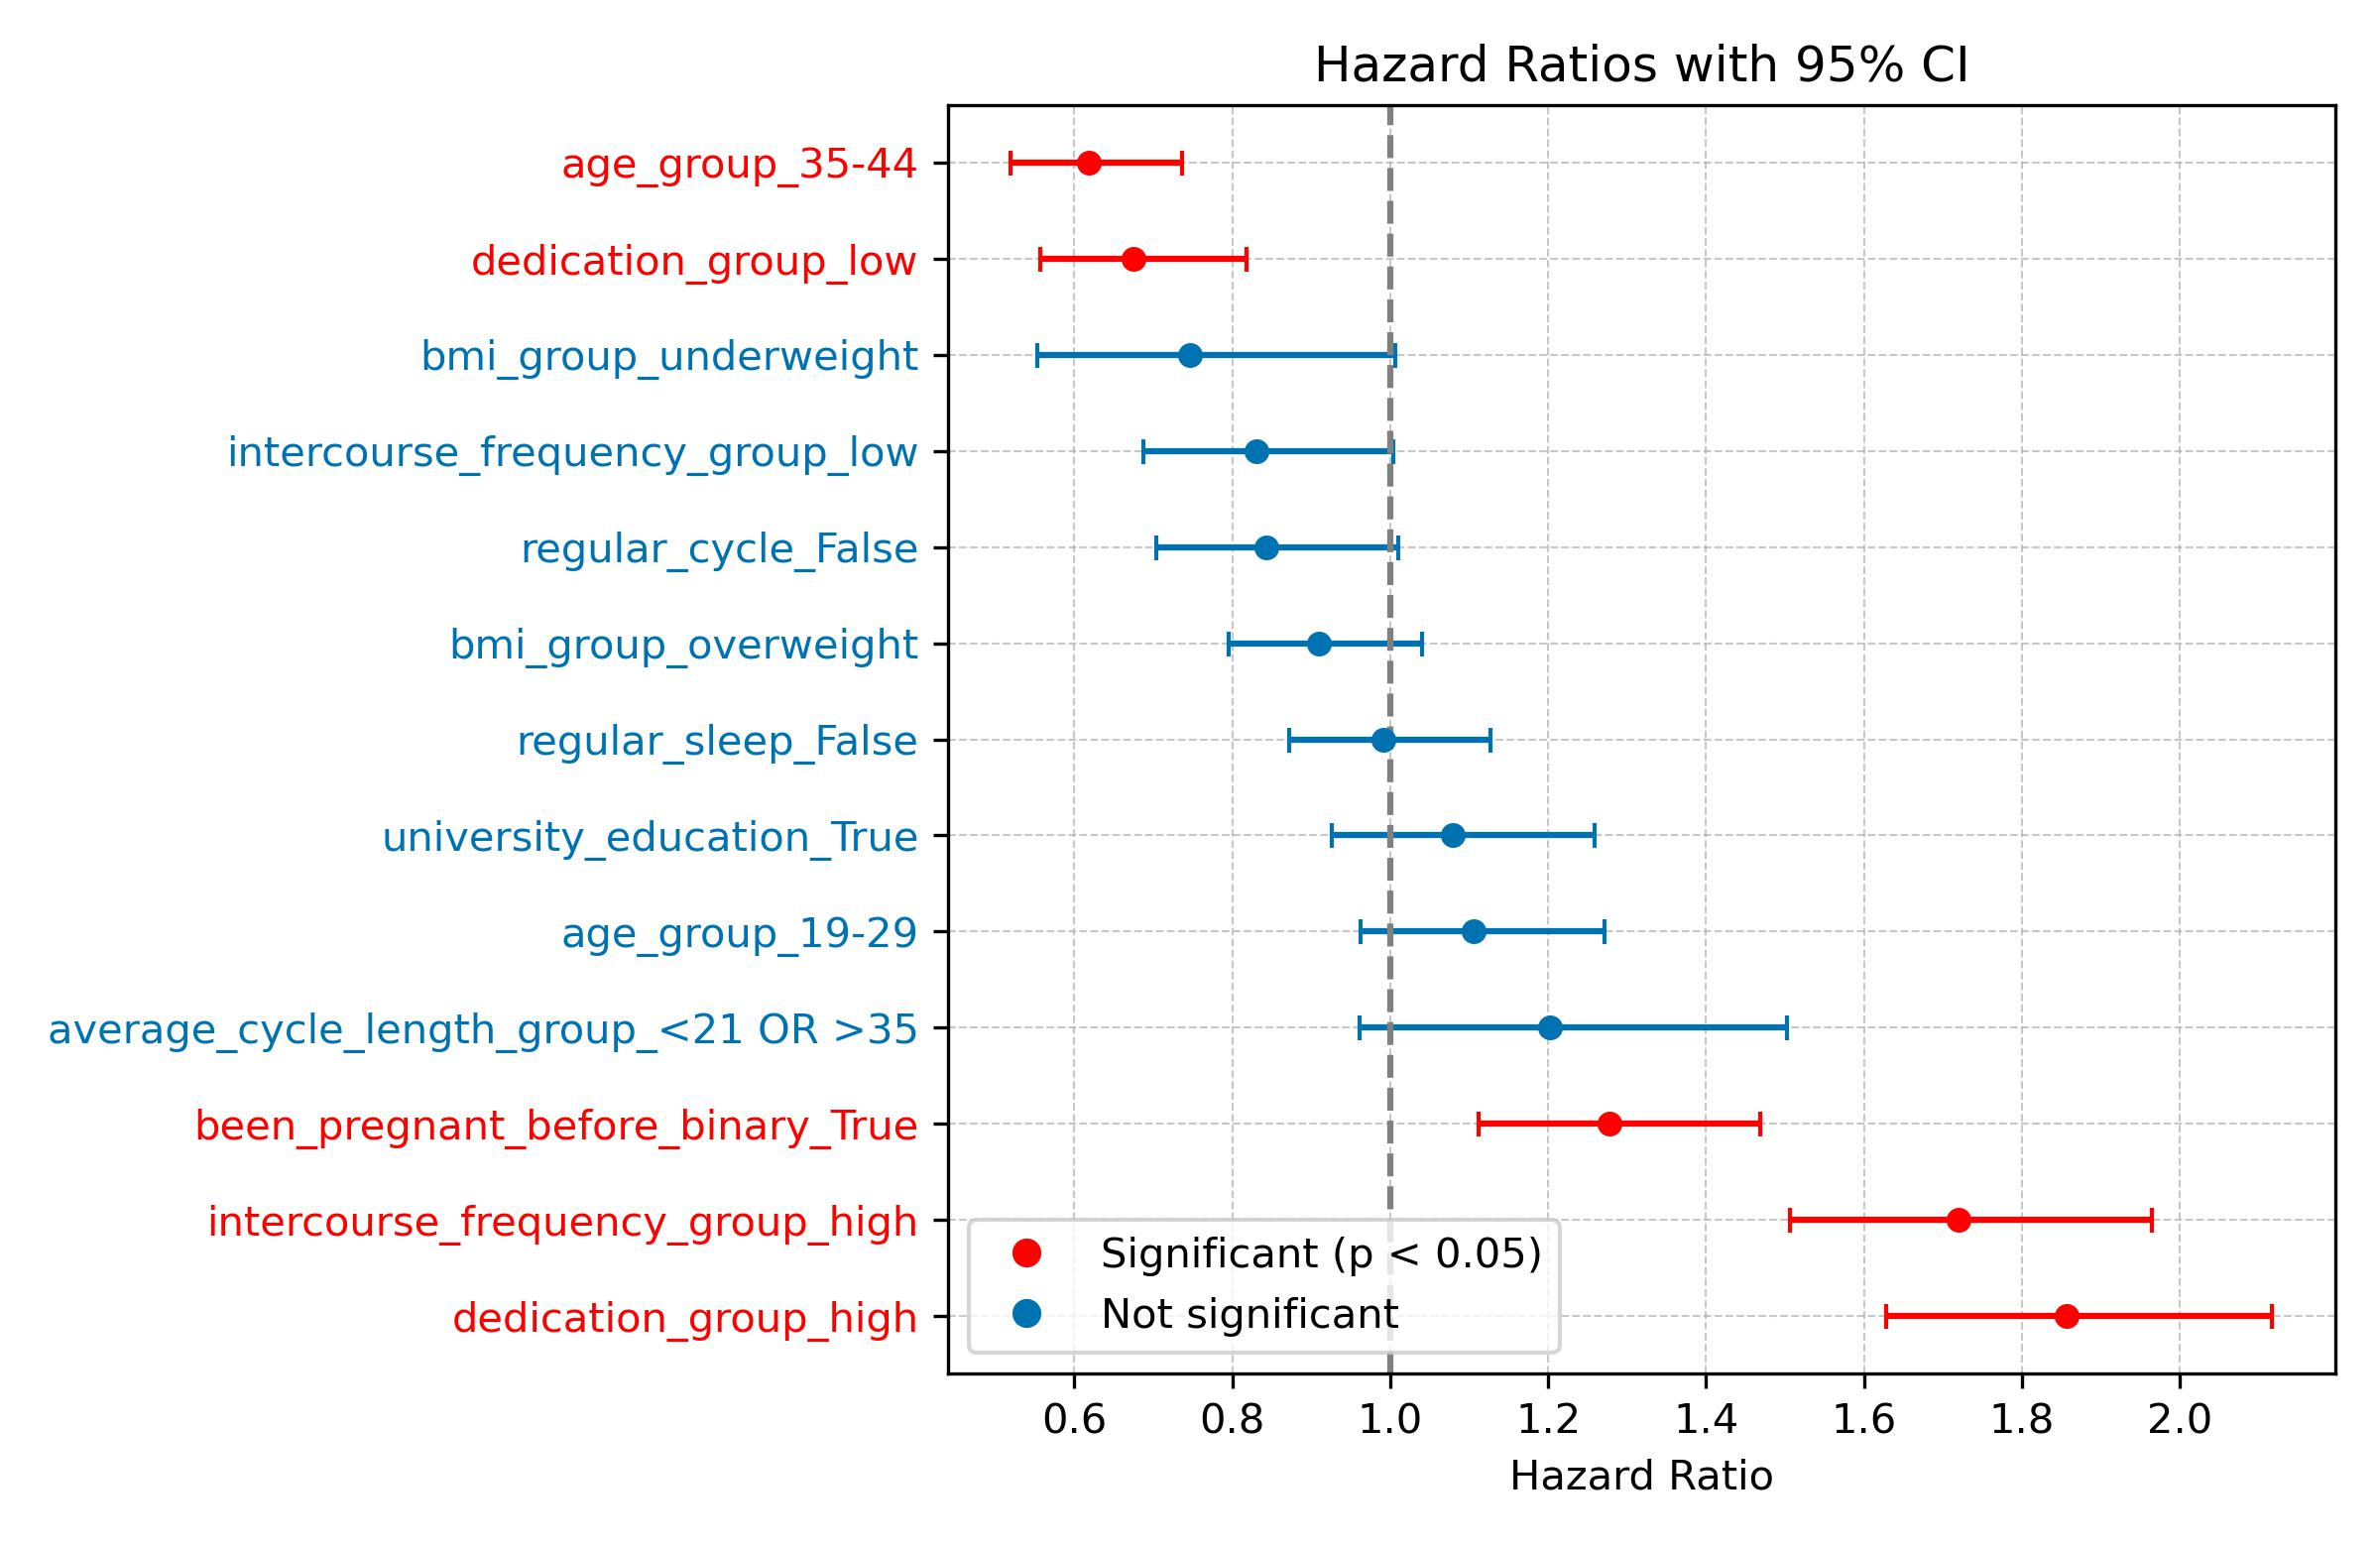
\includegraphics[width=0.65\linewidth]{plots/cox_hr_plot.jpg}
  \caption{
    Hazard ratios for factors potentially affecting time to pregnancy, estimated using a Cox proportional hazards model. Red bars indicate variables with statistically significant effects.\\
  } 
  \label{fig:cox_hr}
\end{SCfigure}

The results are consistent with those obtained from the discrete-time logistic regression model: \textbf{higher age is associated with a lower probability of conception}, while \textbf{previous pregnancies}, \textbf{more dedicated use of the NC app}, and \textbf{higher frequency of logged intercourse} are associated with an increased likelihood of pregnancy.

While an underweight BMI is not statistically significant in this analysis (the 95\% confidence interval includes 1), the estimated hazard ratio is still below 1, suggesting a potential negative association that may not reach significance due to wider CI.



\section{Question 4: Thoughts on Different Techniques}
\label{sec:thoughts}

\questiontext{How would your approach change if you were to use different techniques (e.g., ML or non-ML methods)? What trade-offs would you consider?}

Except for the imputation of missing data, I did not use machine learning (ML) techniques in this assignment. For imputation, I used the \texttt{miceforest} library, which, as described in Section~\ref{sec:other_factors}, applies gradient-boosted trees. I chose this approach because gradient-boosted trees can capture potential non-linear relationships between variables during imputation — something that standard MICE methods cannot.

For Questions 1 and 2, I interpreted the task as an inference problem. From this perspective, I do not think ML would provide meaningful benefits. These are standard time-to-event analyses involving two main variables, where traditional statistical methods offer a robust and well-established framework — particularly for estimating uncertainty.

That said, the questions could also be interpreted differently. For example, “What is the chance of getting pregnant within 13 cycles?” could be read as “What is the chance that a specific NC user gets pregnant within 13 cycles?” In that case, the problem becomes one of individual-level prediction — better suited for ML approaches such as binary classification. However, this would require models capable of handling censored data, such as survival forests or gradient-boosted survival models.

Question 3 presents a somewhat different scenario. Even under my interpretation — a multivariate analysis to assess how different factors influence time to pregnancy — ML techniques could be a valid alternative. In particular, ML approaches might be beneficial when:

\begin{itemize}
    \item The proportional hazards or proportional odds assumptions are violated. Non-parametric models such as \textbf{Random Survival Forests} or \textbf{Gradient Boosted Survival Trees} (e.g., \texttt{XGBoost}, \texttt{LightGBM}) can handle both assumption violations and complex, non-linear relationships.
    \item There are strong non-linear effects or complex interactions between variables. Flexible models like \texttt{DeepSurv} (a neural network–based extension of the Cox model) may also improve the performance in these cases.
\end{itemize}

I considered using an ML-based survival model for Question 3. In the end, I opted for traditional methods because they allow direct estimation of the effect of individual factors on pregnancy probability, along with interpretable confidence intervals.


\section{Possible Improvements}
\label{sec:improvements}

There are several refinements that could improve the analysis, but were not implemented due to time constraints. Some key elements include:

\begin{itemize}
    \item \textbf{Verification of the proportional odds assumption:} This assumption should be tested more rigorously. While a visual inspection (e.g., checking that survival curves do not cross beyond confidence interval bounds) provides a qualitative indication, a more robust approach would involve fitting separate logistic models at each cycle and verifying that the estimated coefficients remain stable within statistical uncertainty.

    \item \textbf{Alternative modeling if assumptions are violated:} If the proportional odds assumption does not hold, it would be advisable to move beyond the discrete-time logistic regression model. Alternatives include non-parametric or ML approaches, as discussed in Section~\ref{sec:thoughts}, or explicitly modeling time interactions (e.g., including terms like \texttt{age}~$\times$~\texttt{cycle}).

    \item \textbf{Accounting for imputation uncertainty:} As mentioned in Section~\ref{sec:other_factors}, the MICE framework can generate multiple imputed datasets. Performing the analysis separately on each and then pooling the results would allow for an estimation of the uncertainty introduced by the imputation process.

    \item \textbf{Reducing model complexity to lower uncertainty:} I included a broad set of factors in the analysis, as it was not clear a priori which would be most influential — although the correlation matrix in Section~\ref{sec:eda} provided useful guidance. However, defining the baseline group across many variables increases model complexity and statistical uncertainty. This could be improved by focusing on the most relevant predictors or by treating some variables (such as \texttt{age} and \texttt{bmi}) as continuous, which would allow more efficient use of the available data.
    
\end{itemize}




\clearpage

\appendix
\section{Overview of Variable Distributions}
\label{app:variables}
%\addcontentsline{toc}{section}{}

This appendix provides an overview of the distributions of all variables used in the analysis, grouped into Figure~\ref{fig:dist_n_cycles} (main outcome variables), Figure~\ref{fig:dist_age} (physiological characteristics), and Figure~\ref{fig:dist_education} (behavioral and contextual factors).



% --- Main Variables ---
\begin{figure}[h]
  \centering
  \begin{subfigure}{0.45\textwidth}
    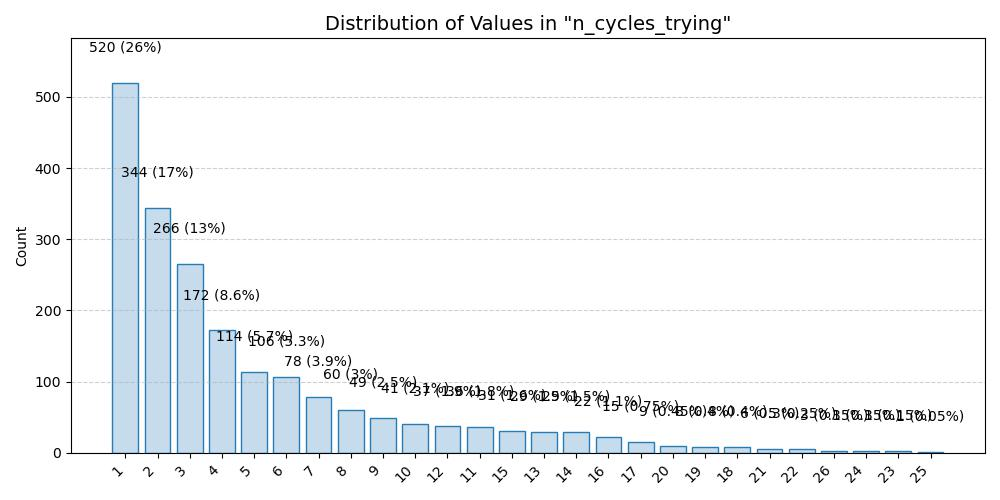
\includegraphics[width=\linewidth]{plots/n_cycles_trying.jpg}
    \caption{Distribution of the number of cycles trying.}
    \label{fig:dist_n_cycles}
  \end{subfigure}
  \hfill
  \begin{subfigure}{0.45\textwidth}
    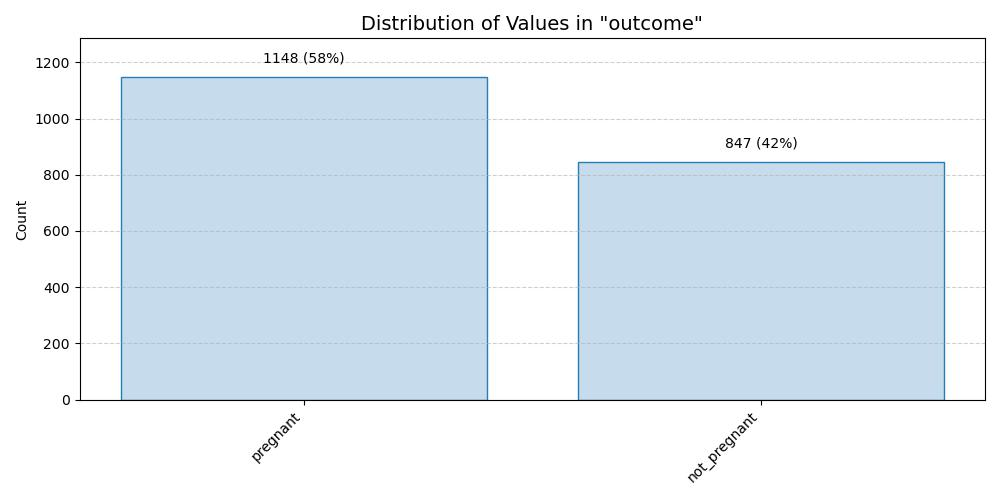
\includegraphics[width=\linewidth]{plots/outcome.jpg}
    \caption{Distribution of pregnancy outcome.}
    \label{fig:dist_outcome}
  \end{subfigure}
  \caption{
    Distributions of main outcome-related variables:
    (\subref{fig:dist_n_cycles}) shows the number of cycles each user tried to conceive before censoring or pregnancy; 
    (\subref{fig:dist_outcome}) shows the binary outcome variable.
  }
\end{figure}

% --- Physiological Characteristics ---
\begin{figure}[h]
  \centering
  \begin{subfigure}{0.45\textwidth}
    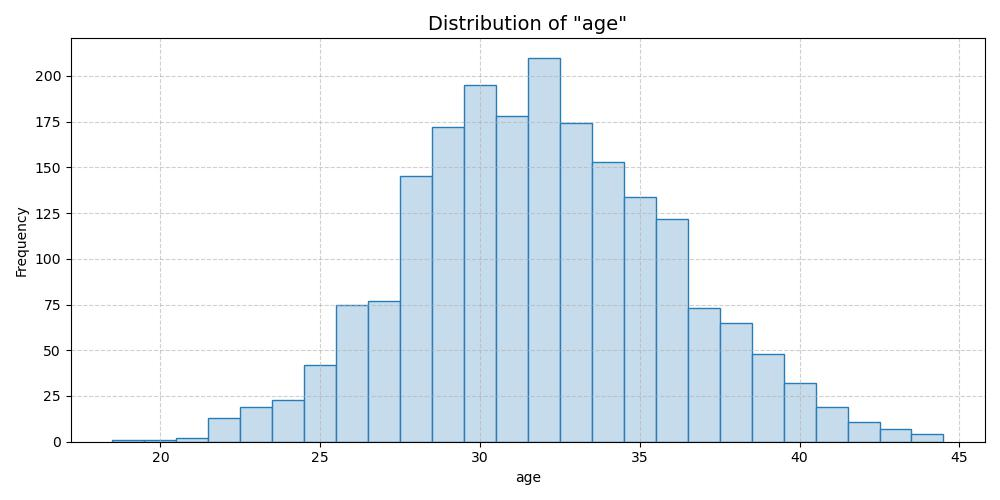
\includegraphics[width=\linewidth]{plots/age.jpg}
    \caption{Age}
    \label{fig:dist_age}
  \end{subfigure}
  \hfill
  \begin{subfigure}{0.45\textwidth}
    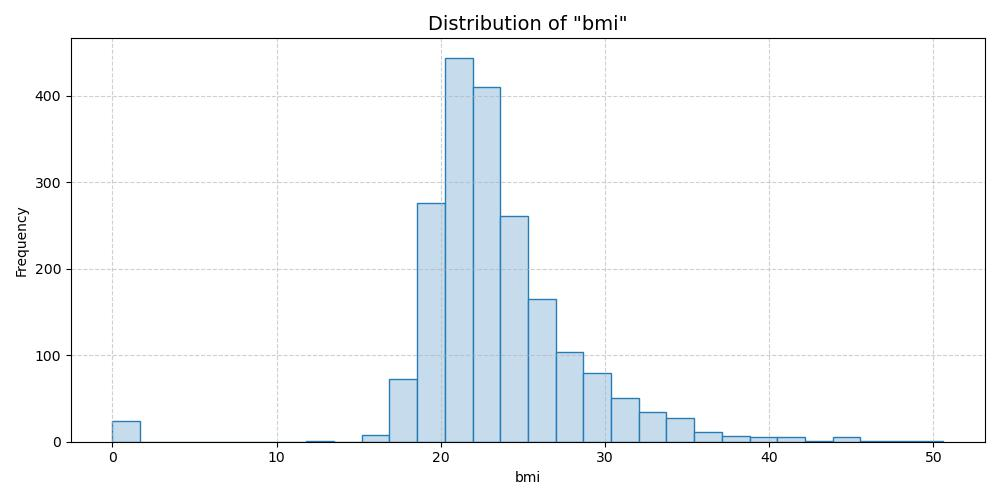
\includegraphics[width=\linewidth]{plots/bmi.jpg}
    \caption{BMI}
    \label{fig:dist_bmi}
  \end{subfigure}
  \\
  \vspace{0.5em}
  \begin{subfigure}{0.45\textwidth}
    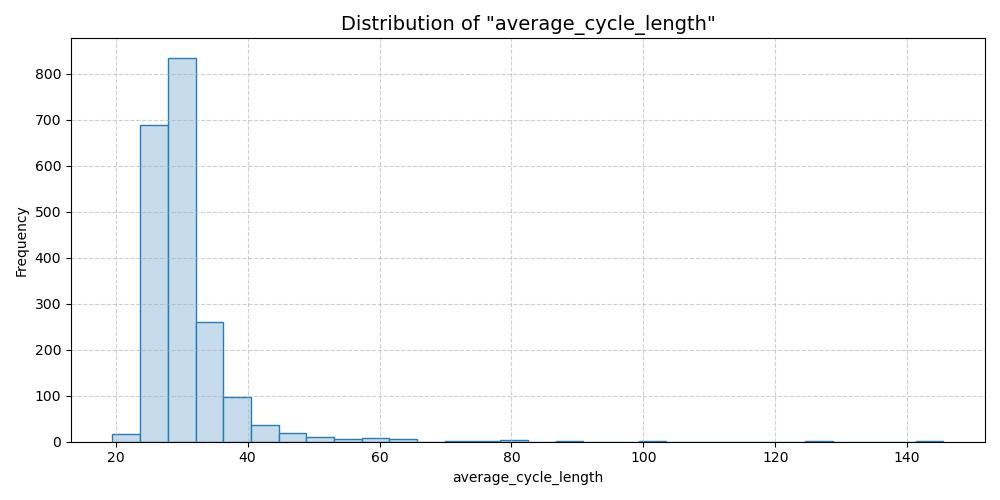
\includegraphics[width=\linewidth]{plots/average_cycle_length.jpg}
    \caption{Average Cycle Length}
    \label{fig:dist_avg_cycle}
  \end{subfigure}
  \hfill
  \begin{subfigure}{0.45\textwidth}
    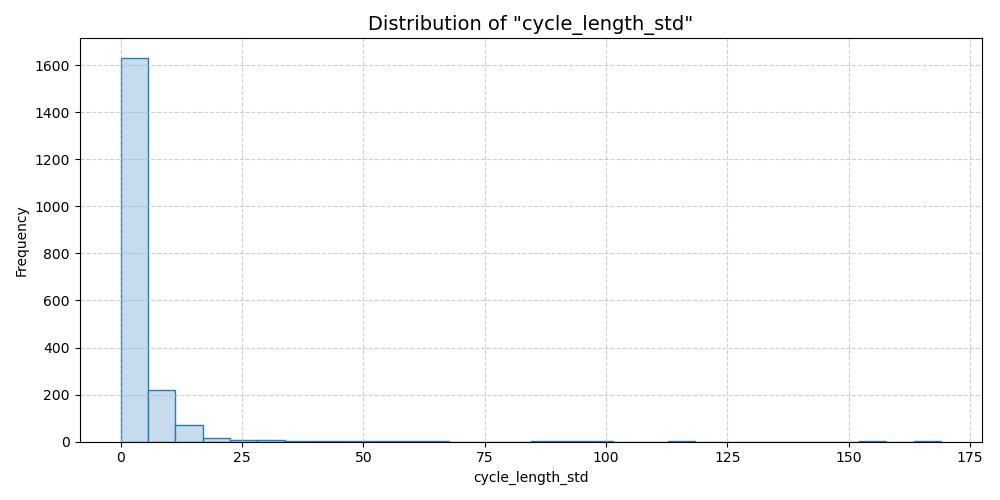
\includegraphics[width=\linewidth]{plots/cycle_length_std.jpg}
    \caption{Cycle Length Variability}
    \label{fig:dist_cycle_std}
  \end{subfigure}
  \\
  \vspace{0.5em}
  \begin{subfigure}{0.45\textwidth}
    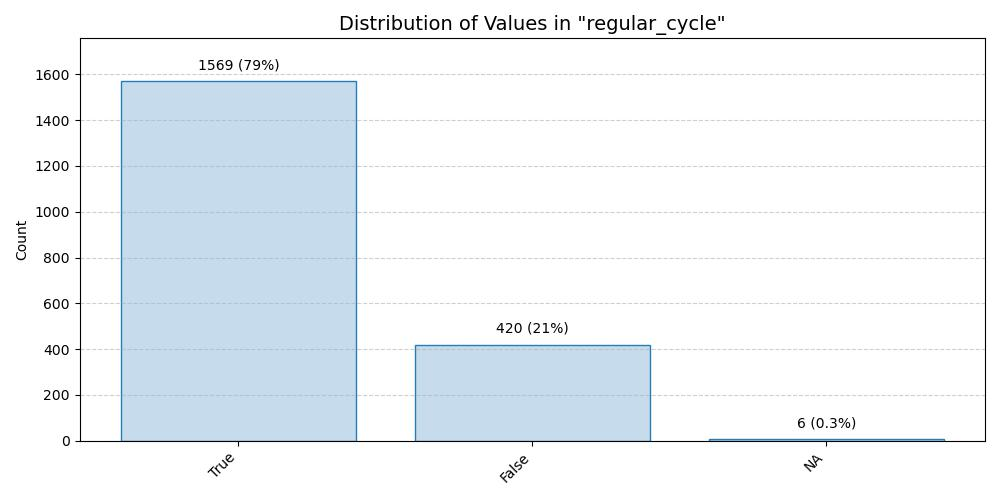
\includegraphics[width=\linewidth]{plots/regular_cycle.jpg}
    \caption{Regular Cycle}
    \label{fig:dist_regular_cycle}
  \end{subfigure}
  \hfill
  \begin{subfigure}{0.45\textwidth}
    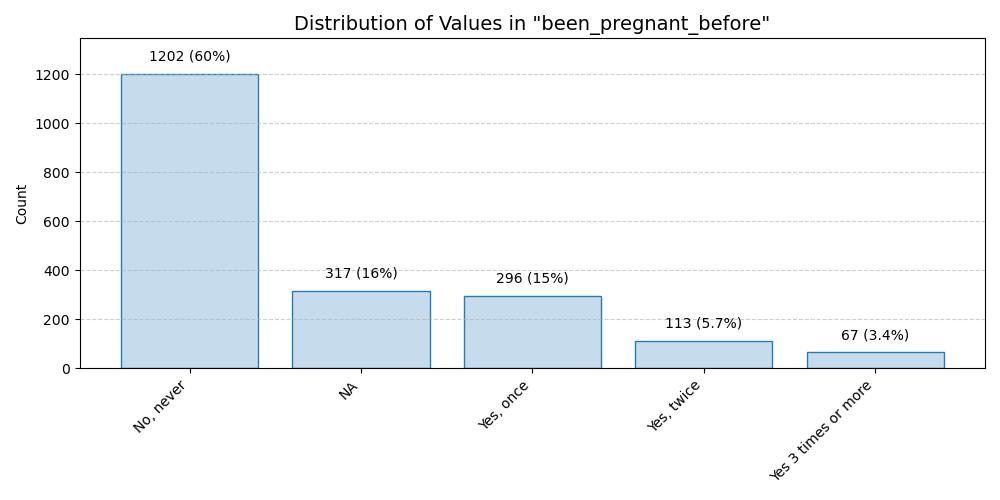
\includegraphics[width=\linewidth]{plots/been_pregnant_before.jpg}
    \caption{Been Pregnant Before}
    \label{fig:dist_prior_preg}
  \end{subfigure}
  \caption{
    Distributions of physiological characteristics: 
    (\subref{fig:dist_age}) age, 
    (\subref{fig:dist_bmi}) BMI, 
    (\subref{fig:dist_avg_cycle}) average cycle length, 
    (\subref{fig:dist_cycle_std}) cycle length variability, 
    (\subref{fig:dist_regular_cycle}) regularity of menstrual cycles, and 
    (\subref{fig:dist_prior_preg}) whether the user had been pregnant before.
  }
\end{figure}

% --- Behavioral and Contextual Factors ---
\begin{figure}[h]
  \centering
  \begin{subfigure}{0.45\textwidth}
    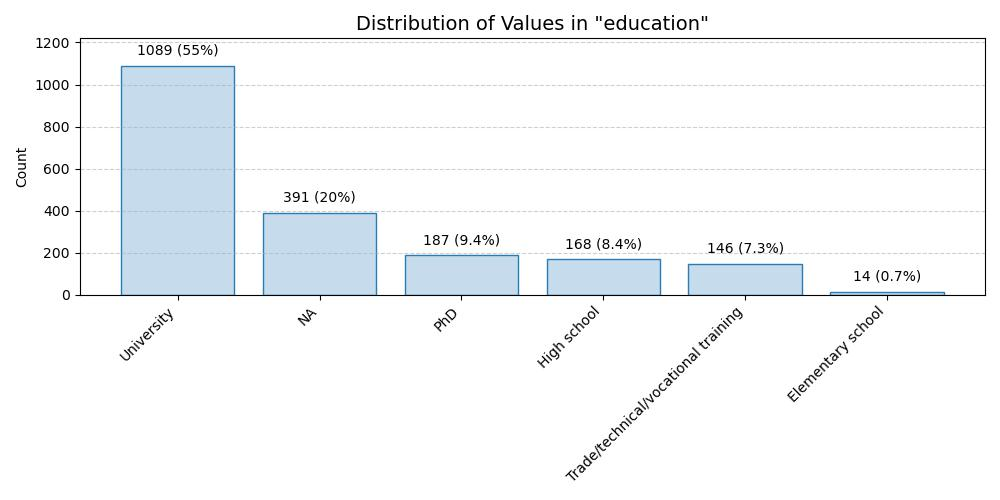
\includegraphics[width=\linewidth]{plots/education.jpg}
    \caption{Education}
    \label{fig:dist_education}
  \end{subfigure}
  \hfill
  \begin{subfigure}{0.45\textwidth}
    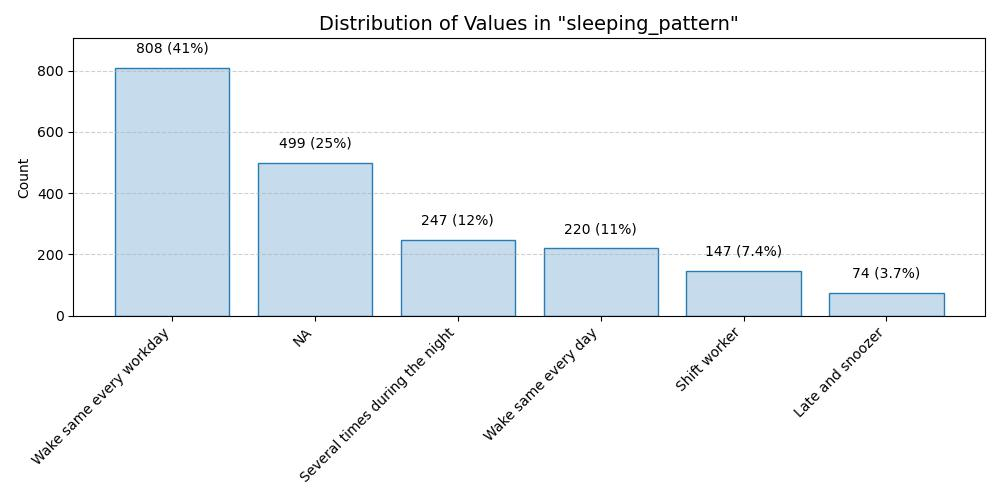
\includegraphics[width=\linewidth]{plots/sleeping_pattern.jpg}
    \caption{Sleeping Pattern}
    \label{fig:dist_sleep}
  \end{subfigure}
  \\
  \vspace{0.5em}
  \begin{subfigure}{0.45\textwidth}
    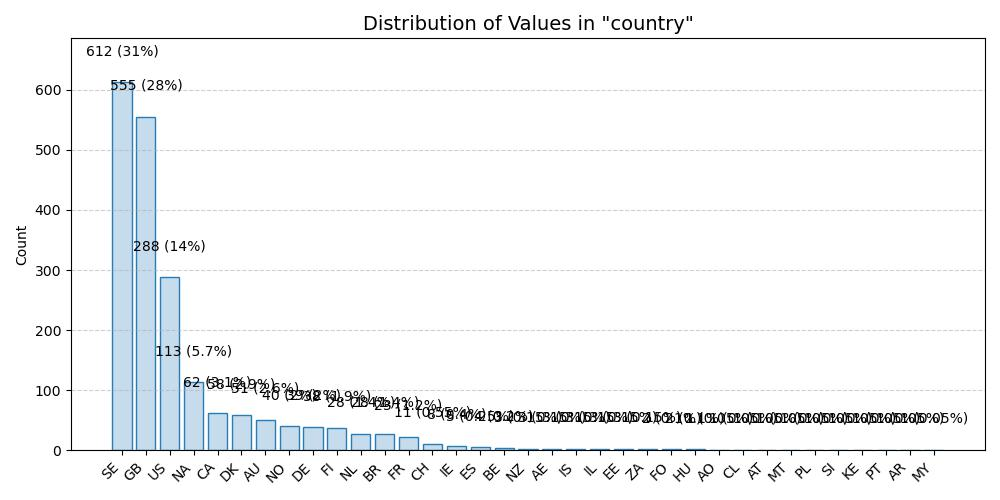
\includegraphics[width=\linewidth]{plots/country.jpg}
    \caption{Country}
    \label{fig:dist_country}
  \end{subfigure}
  \hfill
  \begin{subfigure}{0.45\textwidth}
    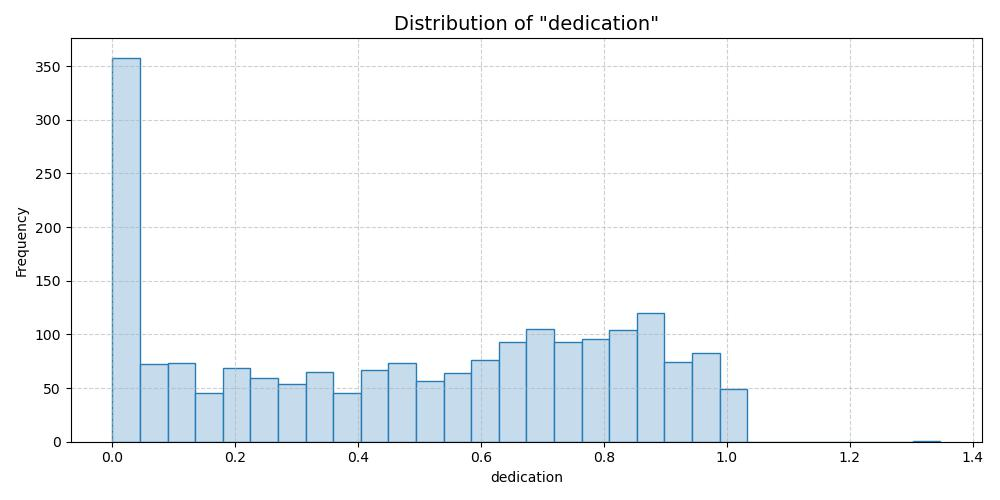
\includegraphics[width=\linewidth]{plots/dedication.jpg}
    \caption{Dedication Score}
    \label{fig:dist_dedication}
  \end{subfigure}
  \\
  \vspace{0.5em}
  \begin{subfigure}{0.45\textwidth}
    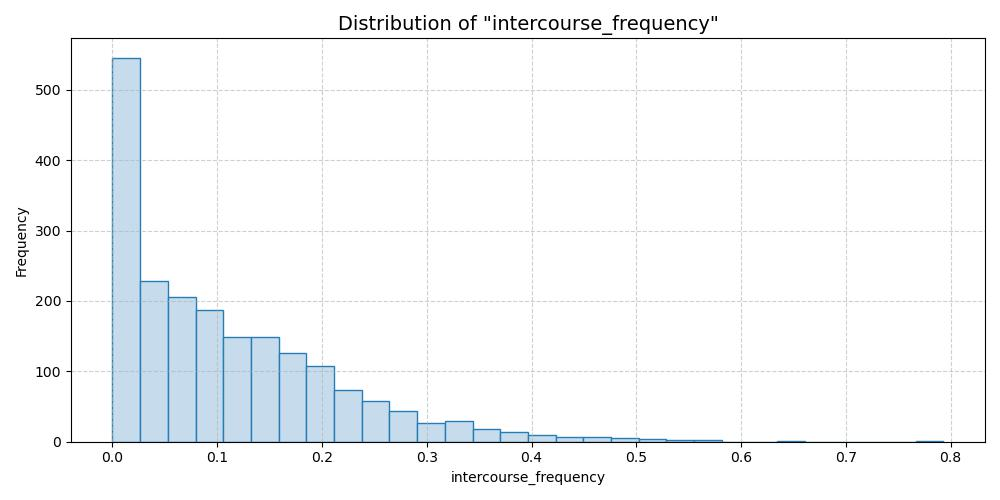
\includegraphics[width=\linewidth]{plots/intercourse_frequency.jpg}
    \caption{Intercourse Frequency}
    \label{fig:dist_intercourse}
  \end{subfigure}
  \caption{
    Distributions of behavioral and contextual variables: 
    (\subref{fig:dist_education}) education level, 
    (\subref{fig:dist_sleep}) sleeping patterns, 
    (\subref{fig:dist_country}) country of residence, 
    (\subref{fig:dist_dedication}) app usage dedication score, and 
    (\subref{fig:dist_intercourse}) reported intercourse frequency.
  }
\end{figure}

\clearpage


\section{Supplemental Material for the Treatment of Missing Values}
\label{app:missing_variables}

This appendix provides additional material related to the treatment of missing values, as discussed in Section~\ref{sec:other_factors}. 

Figure~\ref{fig:or_missing_only} shows the odds ratios estimated using a discrete-time proportional odds regression model applied only to complete cases (i.e., entries with no missing values for the variables considered). This helped identify which variables were relevant and guided the imputation approach. The results can be compared with those in Figure~\ref{fig:or}, obtained after imputation, to confirm that the procedure did not meaningfully distort the final estimates.

Figures~\ref{fig:mf_categorical} and~\ref{fig:mf_continuous} show comparisons between original and imputed distributions for categorical and continuous variables, respectively. These visual checks were used to validate the quality of the imputations. For categorical variables like \texttt{sleeping\_pattern}, \texttt{been\_pregnant\_before}, and \texttt{education}, the distributions after imputation are broadly consistent with those of the observed data. For continuous variables with few missing values, such as \texttt{average\_cycle\_length} and \texttt{cycle\_length\_std}, the comparisons are statistically noisy but show no signs of systematic bias.


\begin{figure}[h]
  \centering
  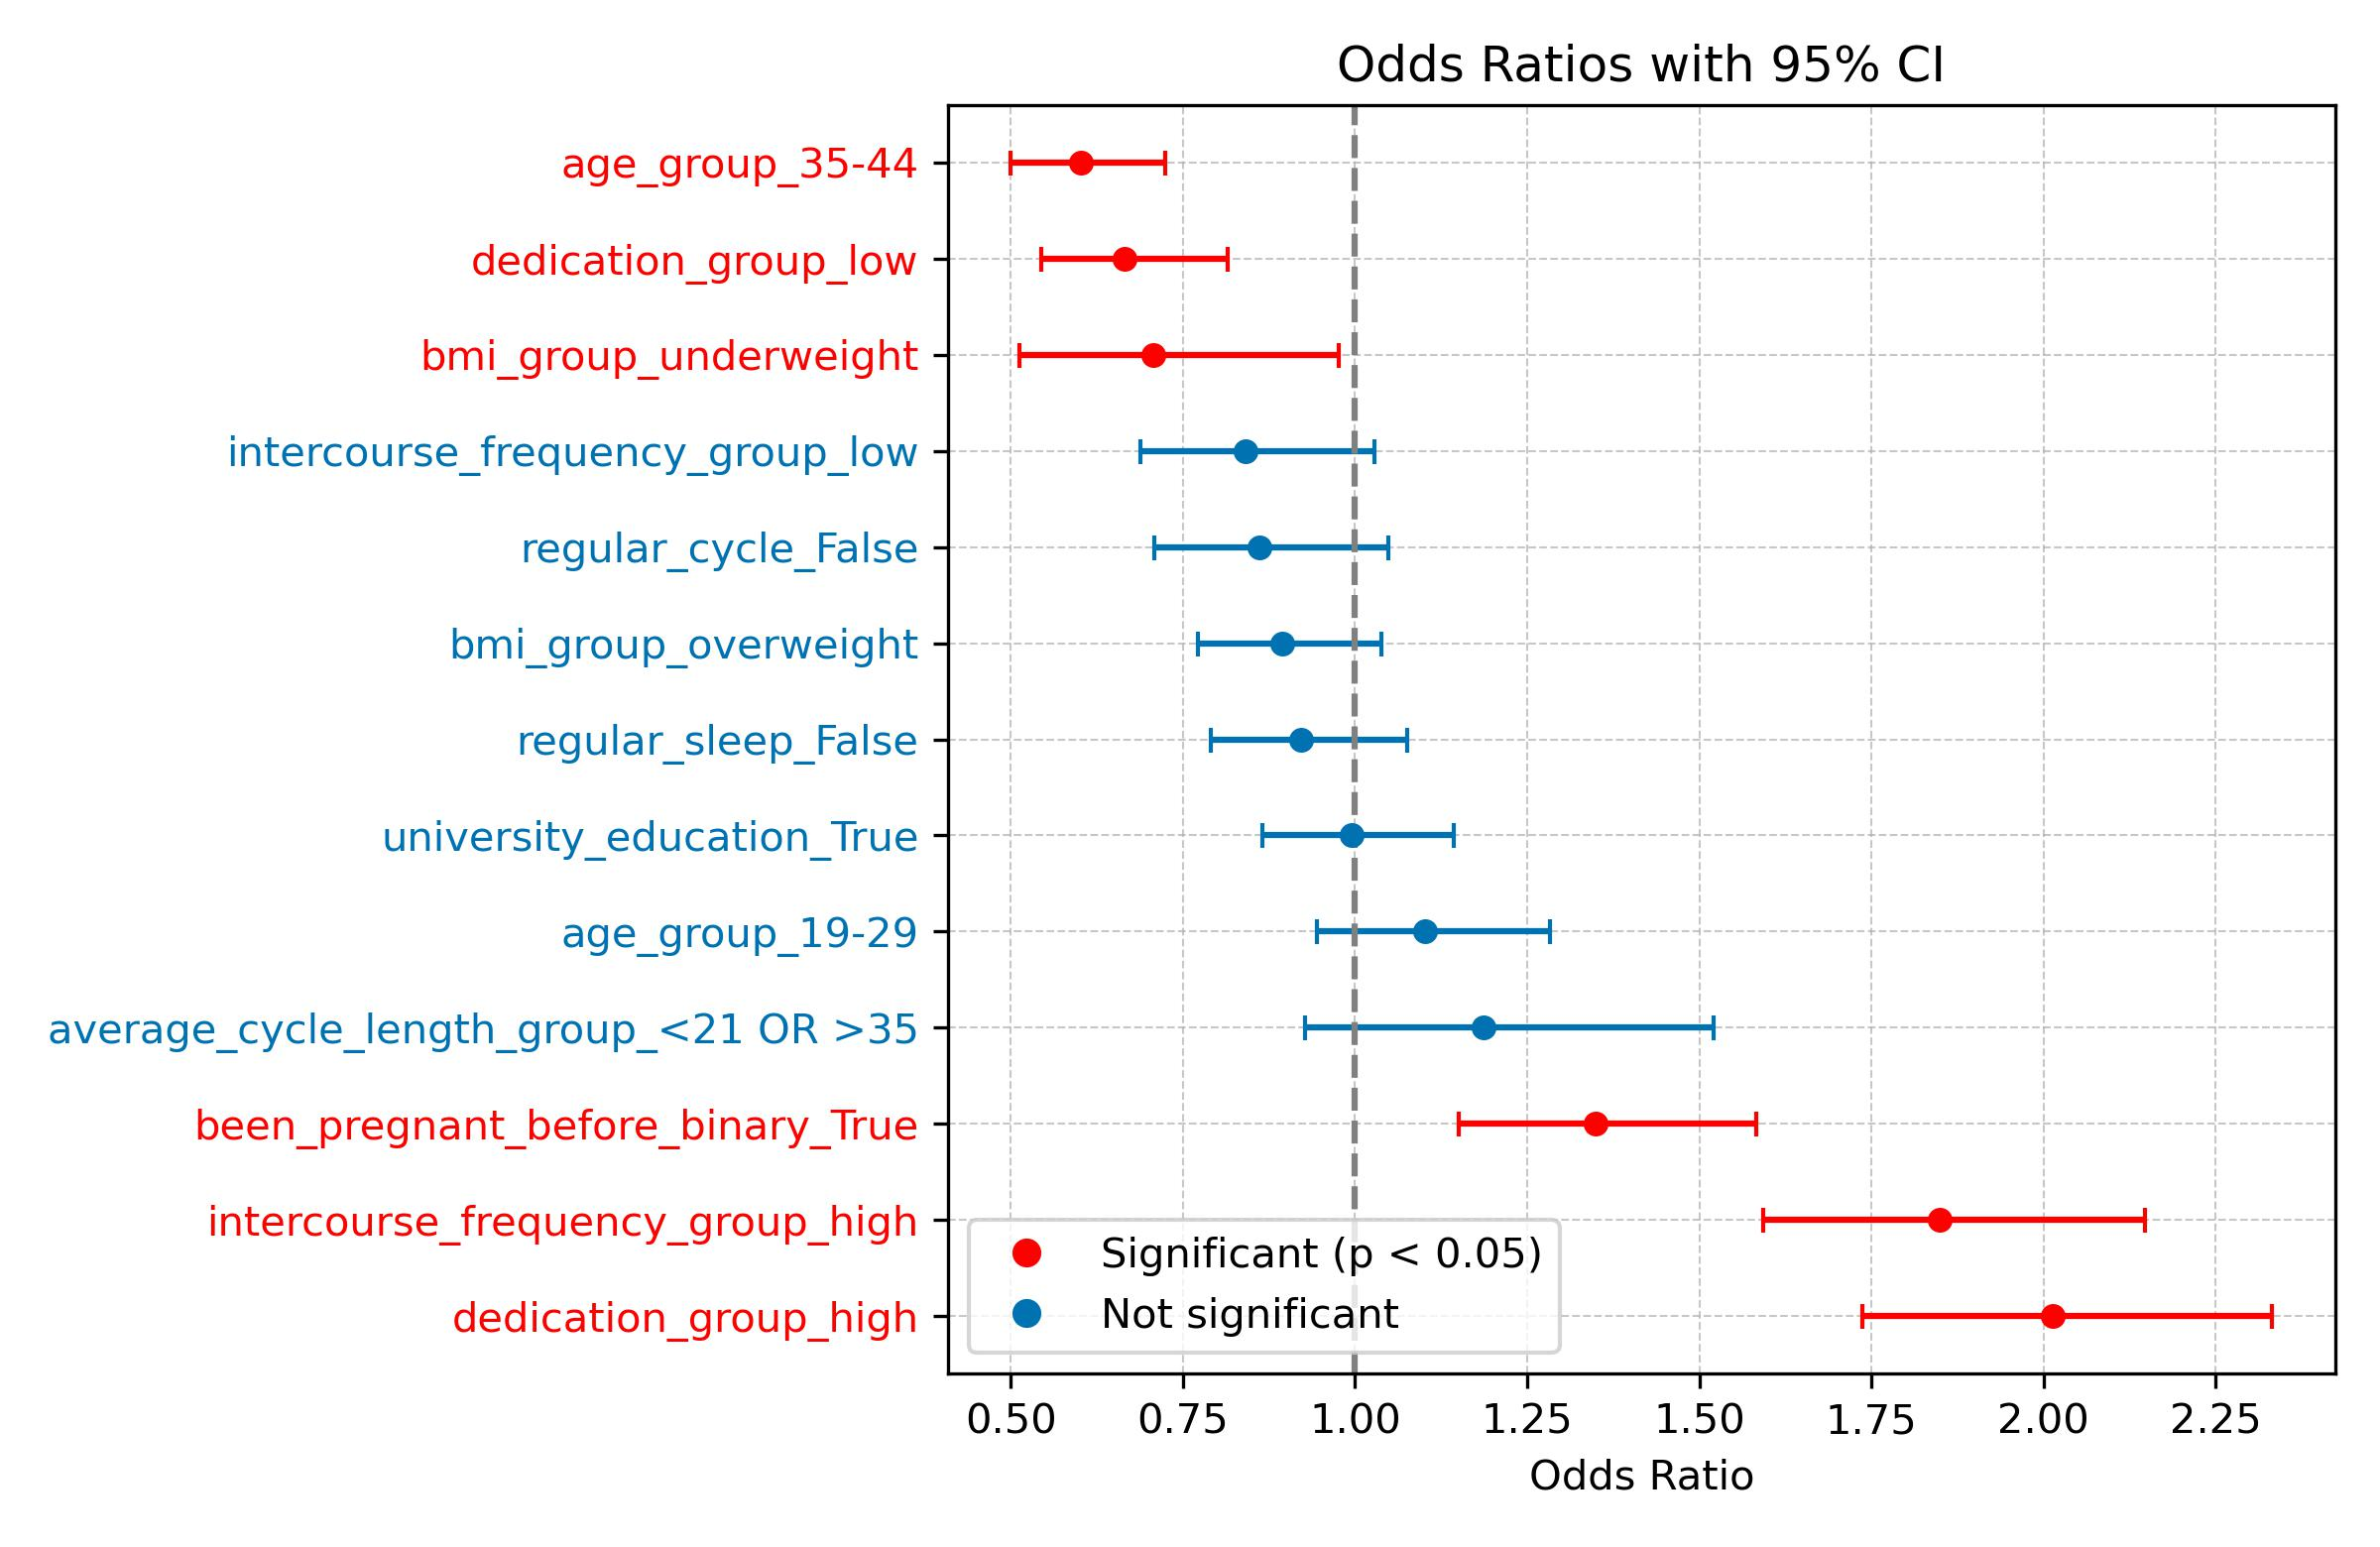
\includegraphics[width=0.65\textwidth]{plots/OR_missing_included.jpg}
  \caption{
    Odds ratios for factors potentially affecting time to pregnancy, estimated using a discrete-time proportional odds regression model. Red bars indicate variables with statistically significant effects. Only data points with no missing variables were included in this analysis.
  }
  \label{fig:or_missing_only}
\end{figure}

\begin{figure}[h]
  \centering
  \begin{subfigure}{0.45\textwidth}
    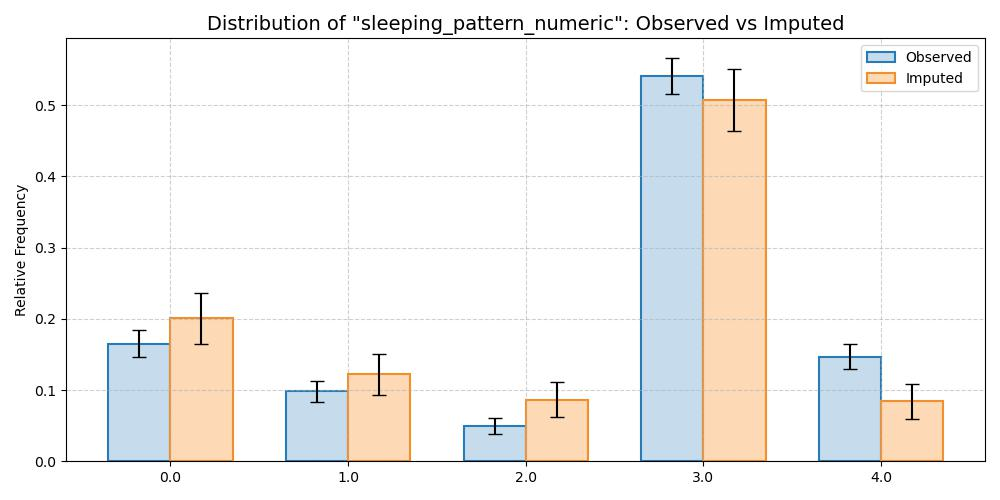
\includegraphics[width=\linewidth]{plots/mf_sleeping_pattern_numeric.jpg}
    \caption{\texttt{sleeping\_pattern}}
    \label{fig:mf_sleeping}
  \end{subfigure}
  \hfill
  \begin{subfigure}{0.45\textwidth}
    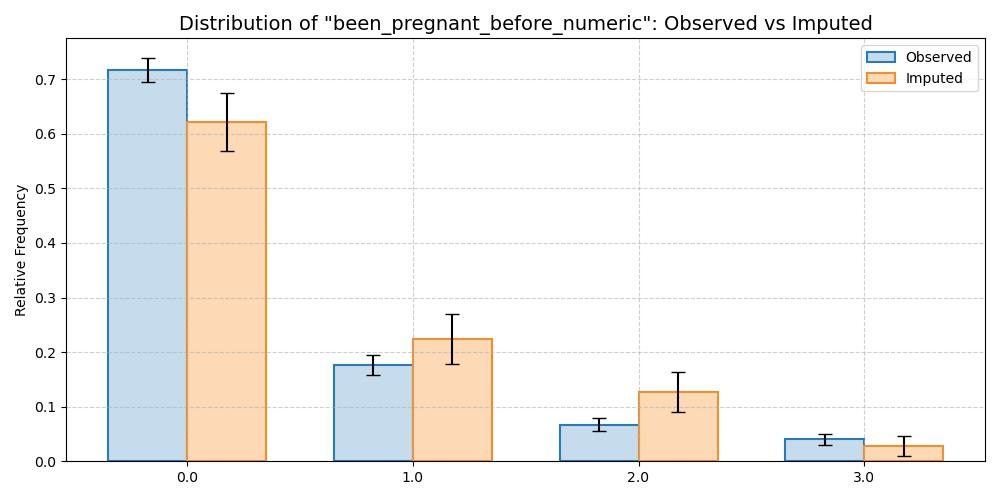
\includegraphics[width=\linewidth]{plots/mf_been_pregnant_before_numeric.jpg}
    \caption{\texttt{been\_pregnant\_before}}
    \label{fig:mf_preg_before}
  \end{subfigure}
  \hfill
  \begin{subfigure}{0.45\textwidth}
    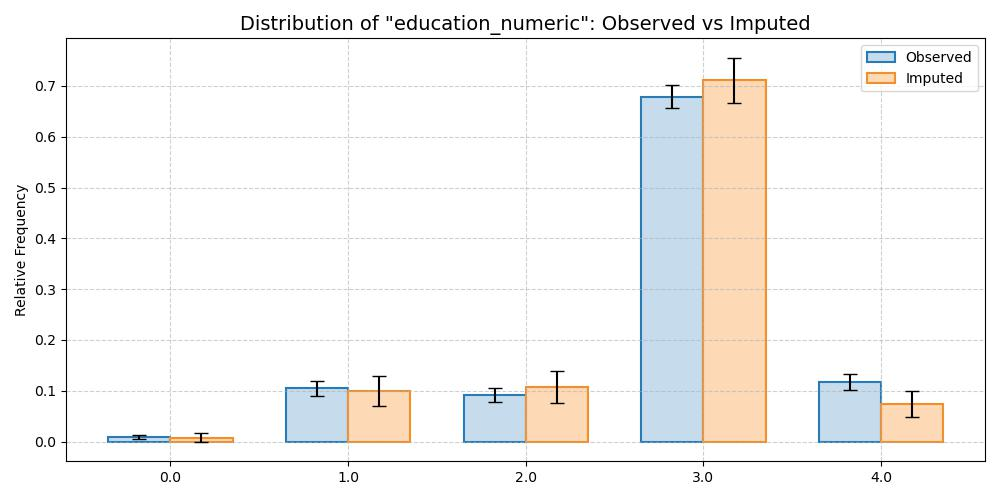
\includegraphics[width=\linewidth]{plots/mf_education_numeric.jpg}
    \caption{\texttt{education}}
    \label{fig:mf_education}
  \end{subfigure}
  \caption{
    Comparison of original and imputed distributions for categorical variables requiring imputation: 
    (\subref{fig:mf_sleeping}) \texttt{sleeping\_pattern}, 
    (\subref{fig:mf_preg_before}) \texttt{been\_pregnant\_before}, and 
    (\subref{fig:mf_education}) \texttt{education}.
  }
  \label{fig:mf_categorical}
\end{figure}

\begin{figure}[h]
  \centering
  \begin{subfigure}{0.45\textwidth}
    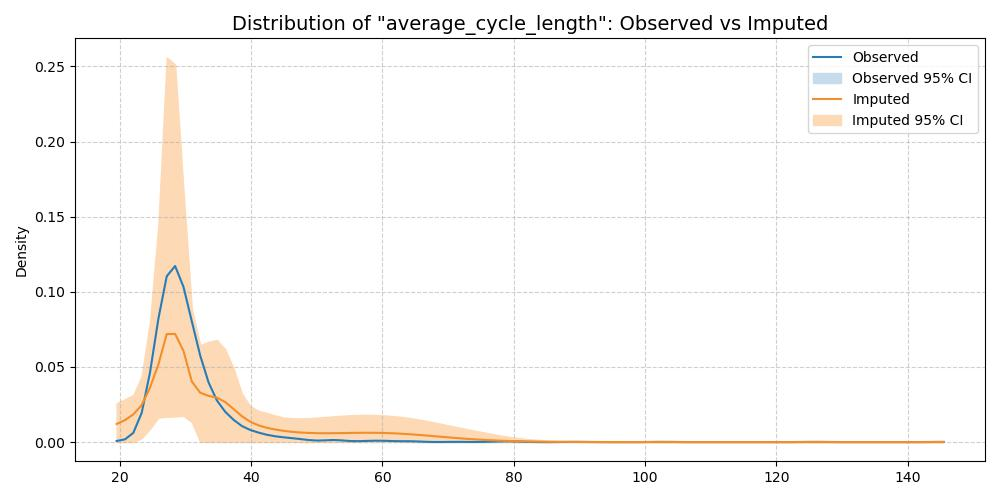
\includegraphics[width=\linewidth]{plots/mf_average_cycle_length.jpg}
    \caption{\texttt{average\_cycle\_length}}
    \label{fig:mf_avg_cycle}
  \end{subfigure}
  \hfill
  \begin{subfigure}{0.45\textwidth}
    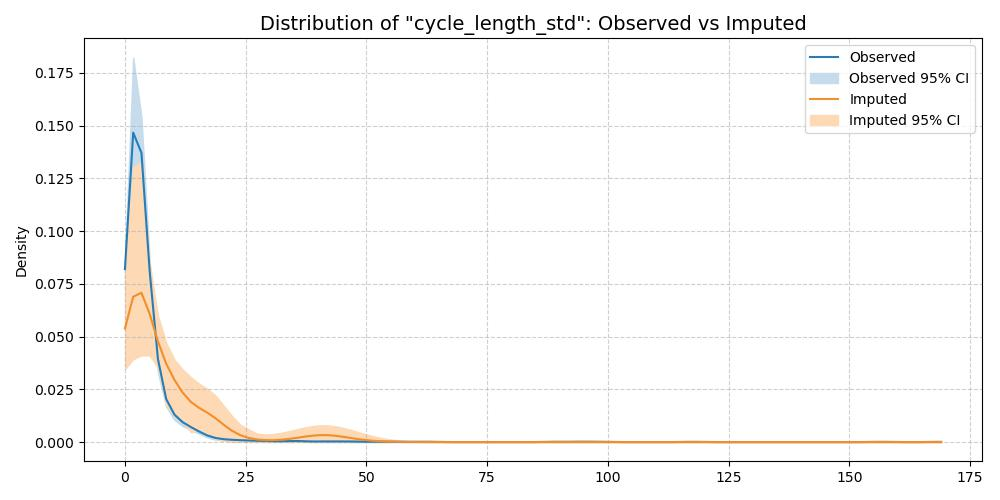
\includegraphics[width=\linewidth]{plots/mf_cycle_length_std.jpg}
    \caption{\texttt{cycle\_length\_std}}
    \label{fig:mf_cycle_std}
  \end{subfigure}
  \caption{
    Comparison of original and imputed distributions for continuous variables with limited missing data: 
    (\subref{fig:mf_avg_cycle}) \texttt{average\_cycle\_length} and 
    (\subref{fig:mf_cycle_std}) \texttt{cycle\_length\_std}. 
    The small number of missing values makes these comparisons statistically noisy, but the imputed distributions appear consistent with the originals.
  }
  \label{fig:mf_continuous}
\end{figure}

\clearpage

\section{Survival Curve Comparisons by Subgroup}
\label{app:survival_subgroups}

This appendix contains Kaplan–Meier survival curves stratified by subgroups of several physiological, behavioral, and socio-demographic factors in the dataset. These plots serve two purposes. First, they provide a visual check of the proportional odds (or hazards) assumption: if survival curves for different groups do not cross beyond their confidence intervals, the assumption is more likely to hold--though this is only a qualitative check and not a formal statistical test. Second, they give an intuitive sense of which variables most strongly affect the time to pregnancy. A steeper drop in the survival function implies a higher probability of pregnancy per cycle.

Figure~\ref{fig:survival_physio} shows the survival curves stratified by physiological and reproductive characteristics: \texttt{age}, \texttt{bmi}, \texttt{average\_cycle\_length}, \texttt{regular\_cycle}, and \texttt{been\_pregnant\_before}. Figure~\ref{fig:survival_behavioral} shows the same analysis for behavioral and socio-demographic factors: \texttt{education}, \texttt{intercourse\_frequency}, \texttt{dedication}, and \texttt{sleeping\_pattern}.

Some patterns are already evident. \textbf{Age}, \textbf{dedication}, and \textbf{frequency of logged intercourse} show strong associations with the probability of pregnancy: younger users, more engaged users, and those with frequent logged intercourse tend to conceive sooner. The survival curves are well-separated and do not cross outside their confidence intervals, suggesting that the proportional odds assumption may be reasonable. One possible exception is \texttt{been\_pregnant\_before}, where lines appear to cross (though still within the confidence bands). This should be verified quantitatively, as discussed in Section~\ref{sec:improvements}.

\vspace{0.5cm}

\begin{figure}[h]
  \centering
  \begin{subfigure}{0.45\textwidth}
    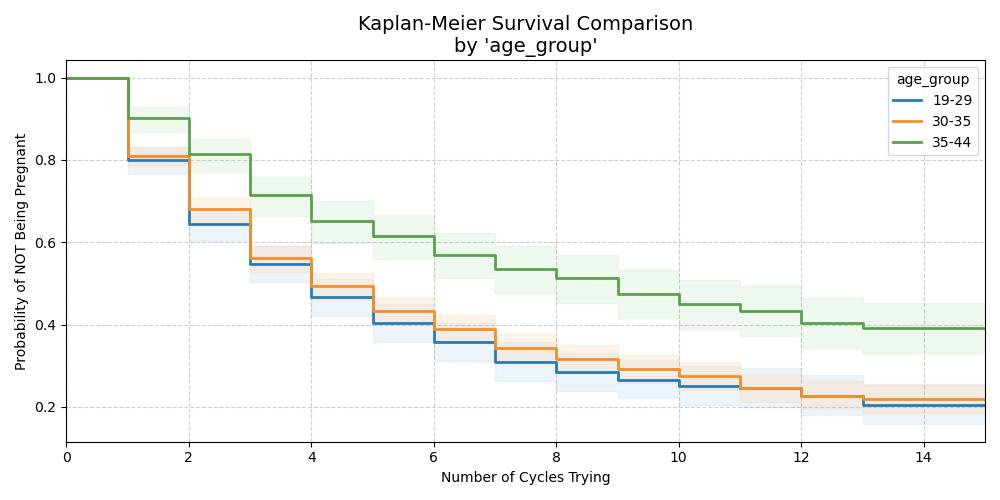
\includegraphics[width=\linewidth]{plots/survival_comparison_age_group.jpg}
    \caption{\texttt{age}}
  \end{subfigure}
  \hfill
  \begin{subfigure}{0.45\textwidth}
    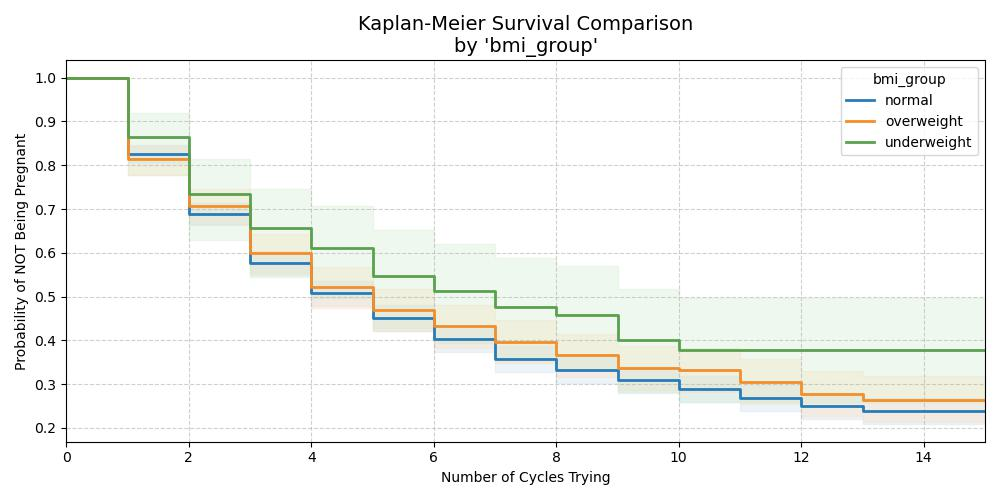
\includegraphics[width=\linewidth]{plots/survival_comparison_bmi_group.jpg}
    \caption{\texttt{bmi}}
  \end{subfigure}

  \vspace{0.3cm}

  \begin{subfigure}{0.45\textwidth}
    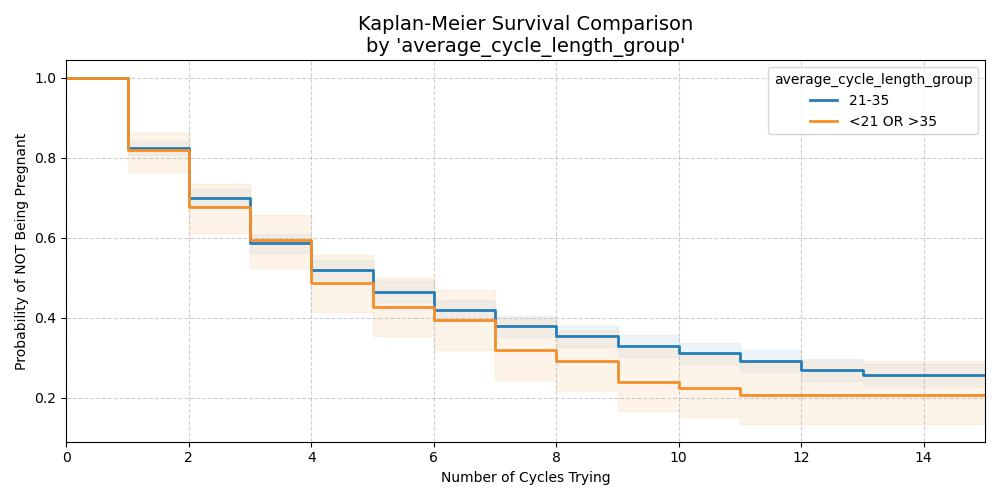
\includegraphics[width=\linewidth]{plots/survival_comparison_average_cycle_length_group.jpg}
    \caption{\texttt{average\_cycle\_length}}
  \end{subfigure}
  \hfill
  \begin{subfigure}{0.45\textwidth}
    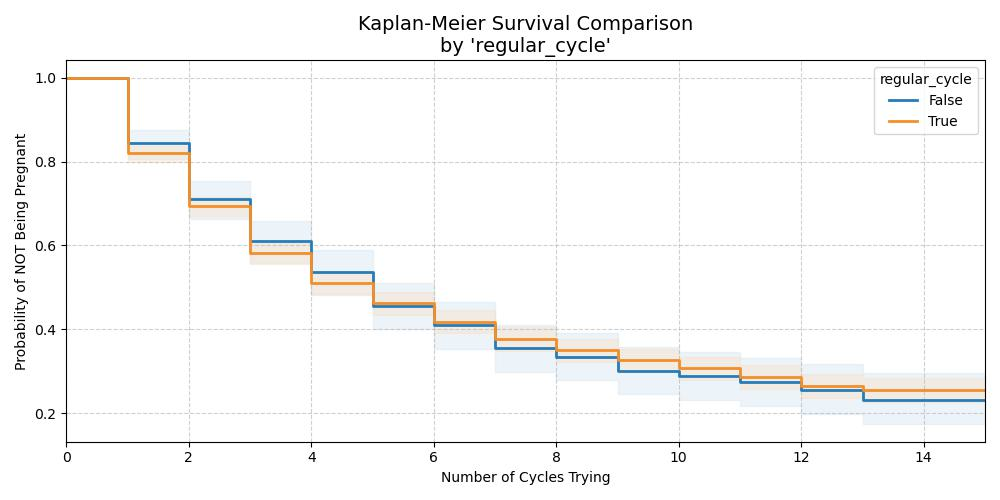
\includegraphics[width=\linewidth]{plots/survival_comparison_regular_cycle.jpg}
    \caption{\texttt{regular\_cycle}}
  \end{subfigure}

  \vspace{0.3cm}

  \begin{subfigure}{0.45\textwidth}
    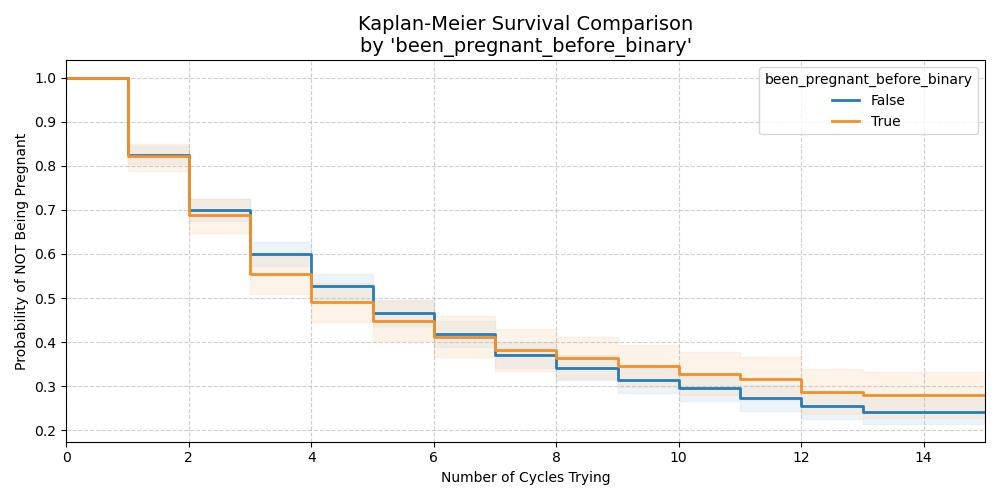
\includegraphics[width=\linewidth]{plots/survival_comparison_been_pregnant_before_binary.jpg}
    \caption{\texttt{been\_pregnant\_before}}
  \end{subfigure}

  \caption{
    Kaplan–Meier survival curves stratified by physiological and reproductive characteristics: 
    (\texttt{age}), (\texttt{bmi}), (\texttt{average\_cycle\_length}), 
    (\texttt{regular\_cycle}), and (\texttt{been\_pregnant\_before}). 
    The shaded areas represent 95\% confidence intervals.
  }
  \label{fig:survival_physio}
\end{figure}

\begin{figure}[h]
  \centering
  \begin{subfigure}{0.45\textwidth}
    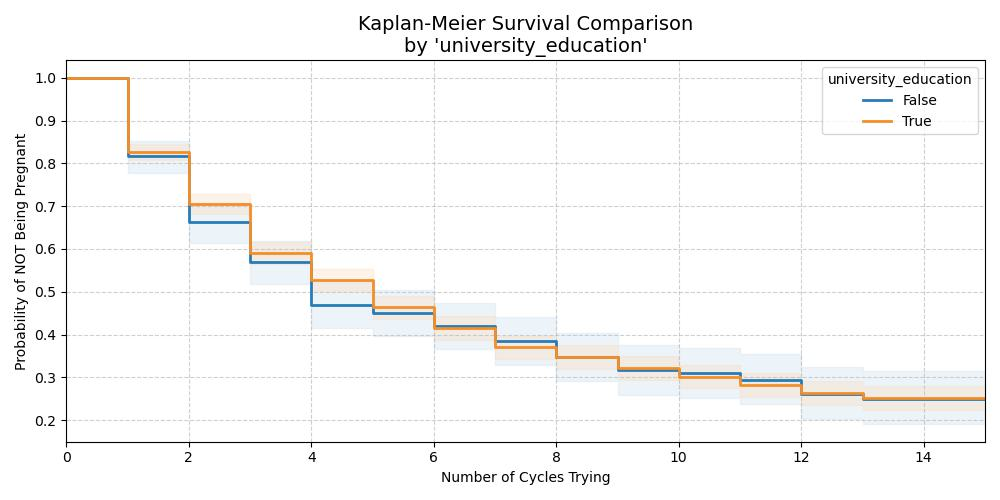
\includegraphics[width=\linewidth]{plots/survival_comparison_university_education.jpg}
    \caption{\texttt{education}}
  \end{subfigure}
  \hfill
  \begin{subfigure}{0.45\textwidth}
    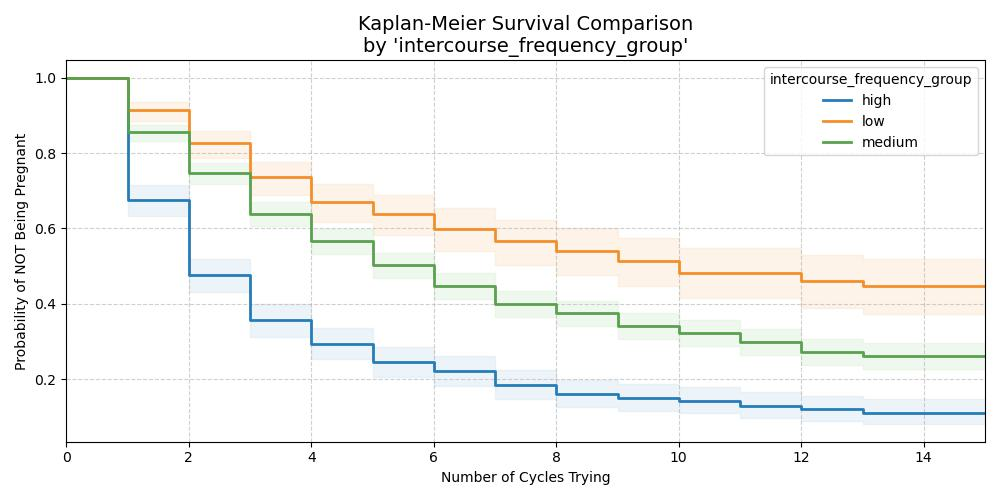
\includegraphics[width=\linewidth]{plots/survival_comparison_intercourse_frequency_group.jpg}
    \caption{\texttt{intercourse\_frequency}}
  \end{subfigure}

  \vspace{0.3cm}

  \begin{subfigure}{0.45\textwidth}
    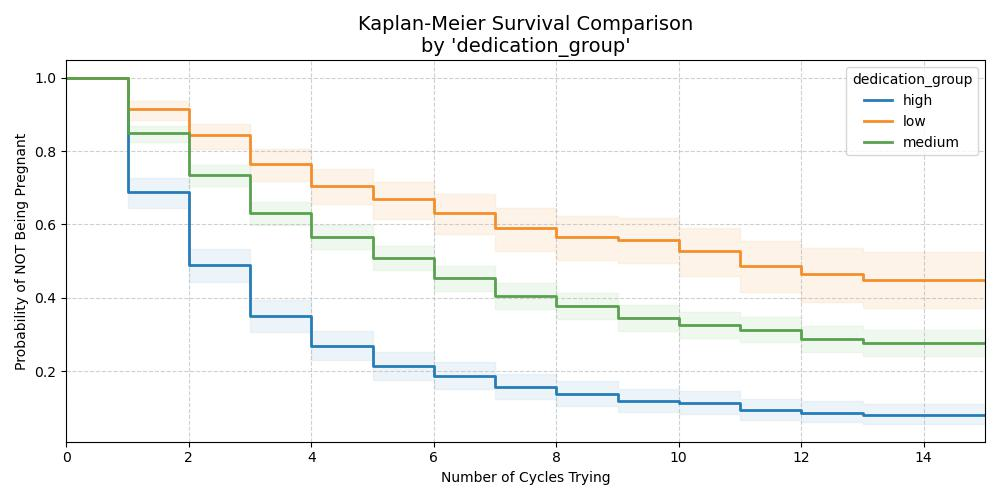
\includegraphics[width=\linewidth]{plots/survival_comparison_dedication_group.jpg}
    \caption{\texttt{dedication}}
  \end{subfigure}
  \hfill
  \begin{subfigure}{0.45\textwidth}
    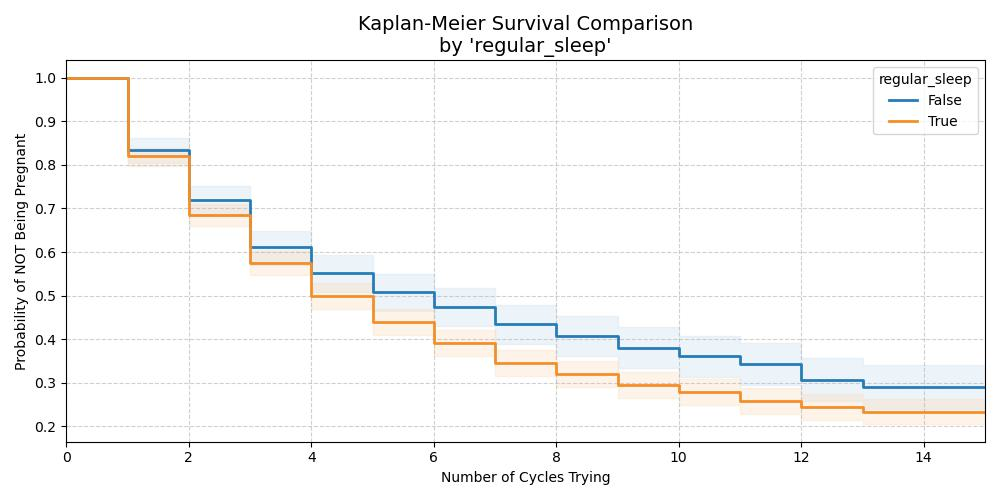
\includegraphics[width=\linewidth]{plots/survival_comparison_regular_sleep.jpg}
    \caption{\texttt{sleeping\_pattern}}
  \end{subfigure}

  \caption{
    Kaplan–Meier survival curves stratified by behavioral and socio-demographic factors: 
    (\texttt{education}), (\texttt{intercourse\_frequency}), (\texttt{dedication}), 
    and (\texttt{sleeping\_pattern}). The shaded areas represent 95\% confidence intervals.
  }
  \label{fig:survival_behavioral}
\end{figure}


\end{document}
